\chapter{Case Studies}\label{ch:case-studies}

\textcolor{red}{FINAL - TO BE READ ONE LAST TIME.}

In this chapter, we investigate our research question (see Section~\ref{sec:prob_rq}) in real world cases through the hypothesis:
\begin{itemize}[leftmargin=42pt]
\item[\textsf{Hp.3}] A solution using \frappe{} conceptual model and an implementation of \river{} computational model, can create a bridge between data analytics and data visualization that enhances the comprehension of a variety of spatio-temporal data and, at the same time, allows reactive decisions.
\end{itemize}

We provide evidence that \textsf{Hp.3} is valid presenting five case studies where we exploited, together, \frappe{} (see Chapter~\ref{ch:conceptual}) and one of the implementations of the \river{} computational model (see Chapter~\ref{ch:computational-impl}) to represent, ingest, augment, synthesize and analyze urban spatio-temporal streaming data.
Section~\ref{sec:cs-mdw} presents our three-years-long experience related to Milano Design Week. Section~\ref{sec:cs-mfw} presents the case study of the Milano Fashion Week and Section~\ref{sec:cs-como} presents the work we carried on for the municipality of Como.

\section{Milano Design Week} \label{sec:cs-mdw}
In the next sections, we report our experience in monitoring Milan Design Week (MDW).
The monitoring project spreads across three editions (2013, 2014 and 2016), and represents a first attempt to put at work a system based on \frappe{}, \sti{}, \hivedi{} and \sparkdi{} to monitor a city-scale event (CSE) that lasts days and is spread across a city.
Indeed, MDW takes place in hundreds of places that host thousands of small-scale events, attracting half a million people.
The aim of the project is to feel the pulse of Milan during the MDW using data from different sources.

\subsection{MDW2013 - Understanding the Data} \label{sec:cs-mdw-2013}
During MDW2013, relying on our past experiences~\cite{DBLP:conf/semweb/BalduiniVDTPC13,DBLP:journals/internet/BalduiniBVHH14}, we concentrate our effort on the social data sources~\cite{pentland2007social}.
We name Social Signal the collection of the digital foot-prints left by MDW attendees on social media. 
During the preliminary study, we recognized that such a signal is strong enough to build a graph linking people, places, and events, but it is not sufficiently reliable (or, more precisely, statistically sound) to identify the most crowded MDW places. 
To tell a reliable story of MDW and identify the most crowded places, we need to show that the social signal is correlated to another, statistically sound, signal. Our hypothesis is that mobile phones can generate such a signal.
We work in partnership with Telecom Italia in order to access privacy preserving aggregates of the mobile phone activity of the people present in Milan area. 
The availability of such a data allows us to compute an index of anomaly that shows off the discrepancies between the expected and the actual activities on the mobile telecommunication network in a given area (for more details, see Section~\ref{sec:comp-mod-eval-cost-prob}).

We study the nature of the social and mobile anomaly signals to understand which visualization better fits the purpose to tell the MDW story to its attendees and we use \frappe{} concepts (marked by special font in the paragraphs) to represent data.

Milan was in overlaid by a square \textsf{Grid} of 10,000 \textsf{Cell}s (100 per side), each of which has a size of 250 x 250 meters. 
We considered three sources of \textsf{Event}s at \textsf{Place}s: mobile phone calls/sms/internet-accesses, geo-referenced micro-posts related to the Milan Design Week, and the 1,200 long-lasting events that are organized in 600 places spread around Milan during the Design Week. 

%In each frame and for each pixel, we count the amount of mobile phone calls, text messages, Internet accesses (namely, mobile phone volume), the amount of the micro-posts on social networks related to the Milan Design Week, the number of Milan Design Week events, and the top hashtags used in each pixels.

The spatial analysis (see Section~\ref{sec:conc-fr-2-analysis}) of the social and telco data, based on \frappe{}, requires to assign each \textsf{OriginalContent} to a specific \textsf{Cell}.

The analysis of the social data requires a mapping action. A social message can be explicitly geo-located and can be easily assigned to a specific \textsf{Cell}, but, more often, a message has no assigned latitude and longitude. In most of the social media posts, related to the MDW, the location can be extracted from the content and linked to the MDW locations exploiting Named Entity recognition and linking techniques during the augmentation phase.

The analysis of mobile phone data is based on CDR (Call Data Record) analysis. CDRs are generated by telecommunication networks to log the activity of the users, associated to a mobile phone cell for billing purposes. Every mobile phone cell has a unique identifier, the Cell Global Identity (CGI). The CGI is characterized by the country, the Mobile Network Operator (MNO), the Location Area of the cell, the latitude and longitude of the barycenter of the cell and of the antenna, the distance between barycenter and antenna, and other properties.
The CDR analysis requires to map each CGI to the \textsf{Cell}s of the \textsf{Grid}.
There are many techniques to do so, we opted for assigning a coverage percentage to each \textsf{Cell} based on the orientation of the antenna, and the land usage of the covered area.

In order to perform a temporal analysis (see Section~\ref{sec:conc-fr-2-analysis}), we captured a \textsf{Frame} every 15 minutes. We did so, because we empirically observed that there is always at least a micropost per \textsf{Frame} -- the social signal is less dense than the telco one.

We analyzed 2 months of CRDs from Milan to synthesize two Gaussian models for each cell (for further details see Section~\ref{sec:comp-mod-eval-cost-prob}): one grouping the \textsf{Frame}s by working days, and one grouping them by week-end days. We were able to build 1.92 millions Gaussian models\footnote{4 frames per hour X 24 hours X 2 day types (working and weed-end days) X 10.000 pixels.}.
The anomaly index is obtained by computing how far the number of calls/sms/internet-accesses (which we refer as $n$) is from the average behavior (which we refer as $avg$), keeping into account the computed
standard deviation (which we refer as $std$). The formula to obtain the anomaly index can be compactly written as:
\[
2\Phi_{avg,std^2} (n) - 1
\]
where $ 2\Phi_{avg,std^2} $ is the cumulative distribution function of a Gaussian random variable with mean $avg$ and variance $std$.
Anomalies are identified by filtering all the records with an anomaly index greater than a given threshold.

\begin{figure}[t]
\begin{center}
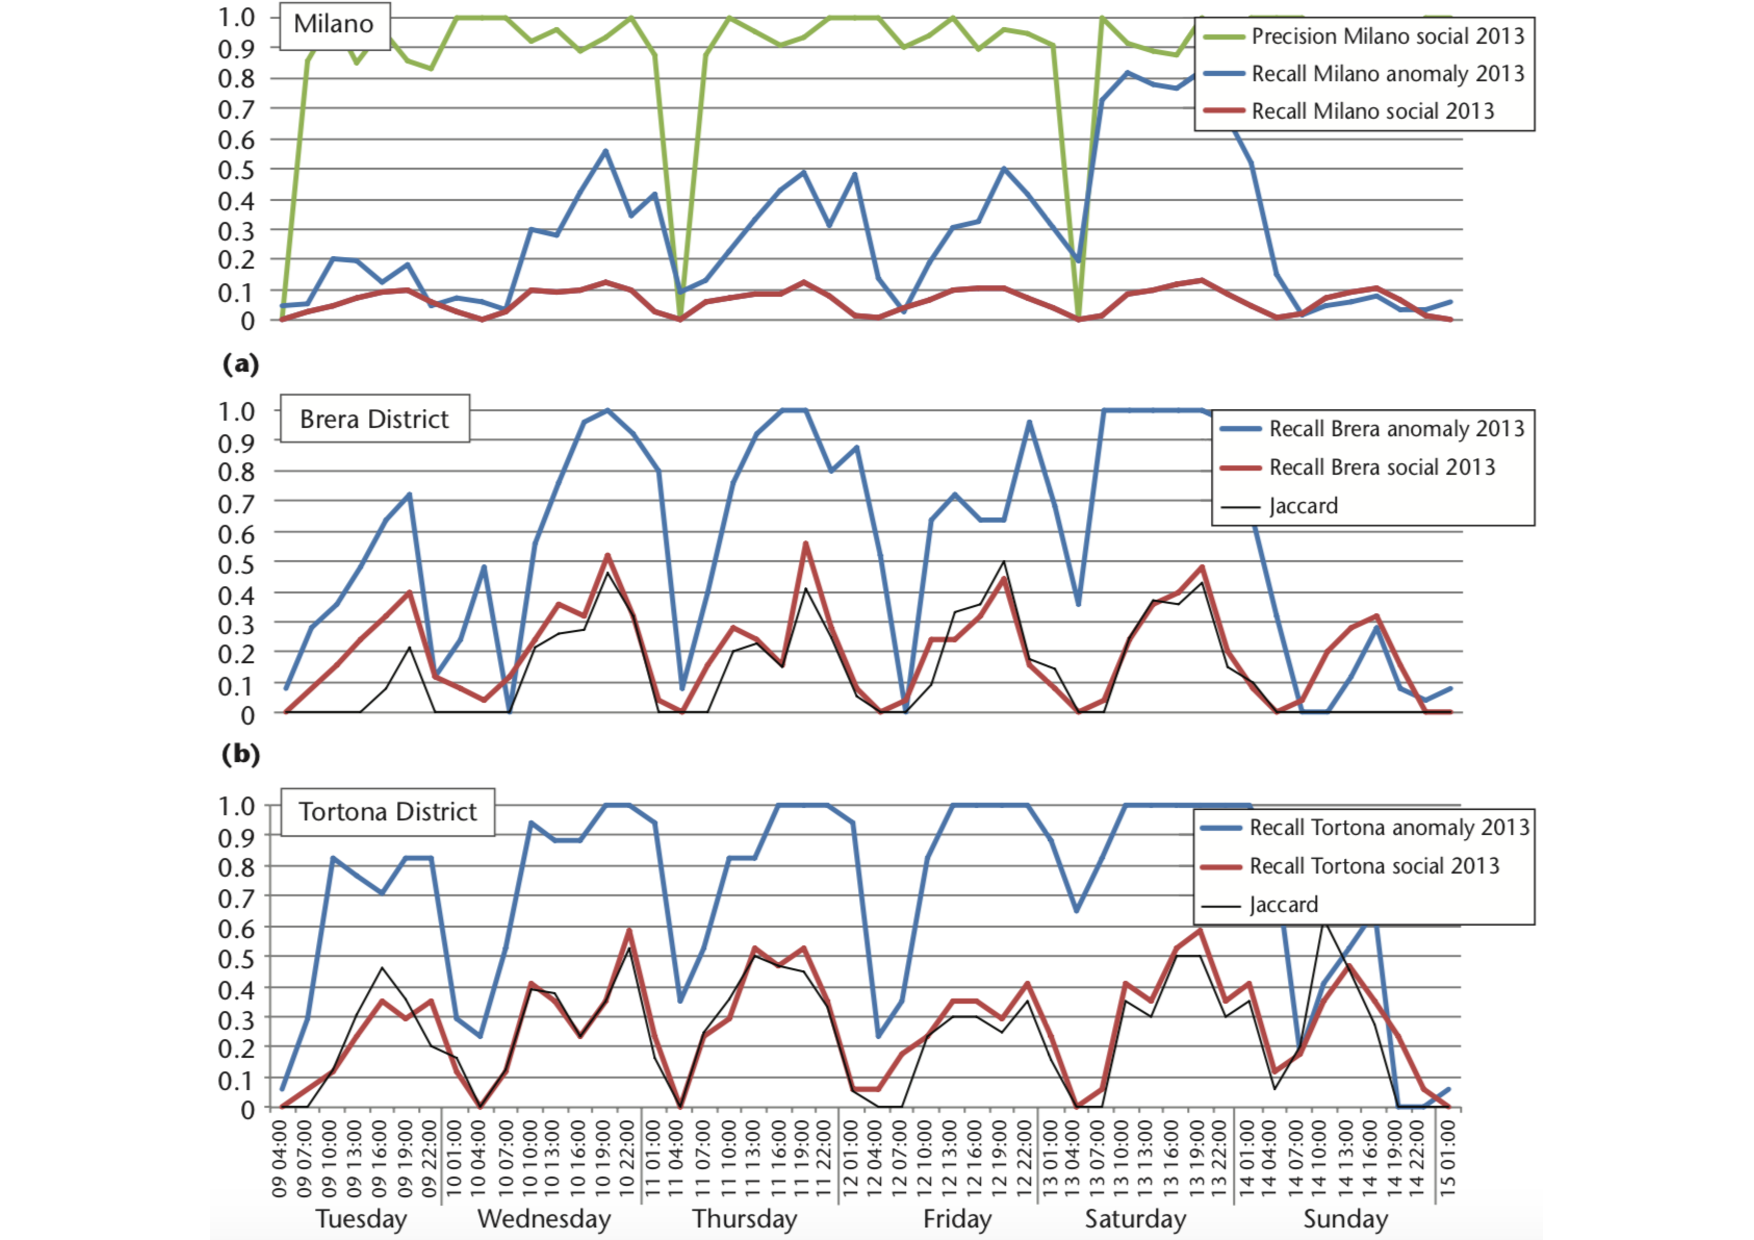
\includegraphics[width=0.90\textwidth]{img/mdw-prec-rec} 
\caption{Precision and recall of the social and mobile anomaly signals in identifying pixels where Milan Design Week (MDW) events happen in (a) Milano and the (b) Brera and (c) Tortona districts.}
\label{fig:mdw-prec-rec}
\end{center}
\end{figure}

We, then, created a gold standard (MilanP) consisting of all the pixels that contain at least one MDW2013 place. We also created two subsets of this gold standard (BreraP and TortonaP) that focus on the pixels that belong to the districts of Brera and Tortona, where the most important events were located. 
For each frame, we measured the ability of the social and mobile anomaly signals in identifying pixels in MilanP, BreraP, and TortonaP (see Figure~\ref{fig:mdw-prec-rec}) measuring precision and recall.

The results of the analysis show that the social signal has high precision (between 0.8 and 1 for 95 percent of the frames) in identifying pixels in MilanP. Its recall is low in identifying pixels in MilanP, but it is good (above 0.4 for around 60 percent of the frames) in identifying pixels in BreraP and TortonaP. In all cases, the signal volume is low: the average number of microposts linked to MDW per hour is 15 for MilanP, three for BreraP, and five for TortonaP.
However, the social signal is correlated to the anomaly index signal (see Figure~\ref{fig:mdw-prec-rec}) during the working days. The Pearson correlation for MilanP is 0.61 with a p-value of 2x$10^{-4}$ for BreraP, it is 0.76 with a p-value of 4.6x$10^{-7}$; and for TortonaP, it is 0.56 with a p-value of 3.1x$10^{-5}$. 

Moreover, not only the two signals are correlated, but they also identify the same pixels. To measure this, we computed the Jaccard similarity coefficient\footnote{The Jaccard coefficient measures similarity between finite sample sets} between the pixels identified by the social signal and those identified by the mobile anomaly signal. 
As we can observe in Figure~\ref{fig:mdw-prec-rec}, the Jaccard similarity coefficients in Brera and Tortona almost constantly overlaps with the recall of the social signal -- that is, if a pixel is identified by the social signal, then it's among those identified by the mobile anomaly signal.

%As a last step in understanding the data, we analyzed the graph that links people, places, and events. Similar to many other graphs describing real-world phenomena, it is scale-free~\cite{price1976general}. The frequency with which places, events, and hashtags of MDW are co-mentioned by people in microposts almost perfectly fits a power law ($y=12289x^{-1.832}$ with $R^2=0.96173$). For this reason, we draw the hypothesis that this information is best visualized using a graph~\cite{bertin1983semiology} where users are nodes, and links between two nodes represent discussions about the same place or event.

The data analysis phase (see phase~3 of the reference architecture presented in Section~\ref{sec:comp-mod-sol-arch}) bring evidences that: (i) Telco Big Data can provide a very relevant and dynamic overview of the presence of people in the context of a specific city or territory, aggregated at the level of the single cell tower, and (ii) Social data represent a precious source to build the interaction graph between people, events and places. 
However, since building the morphology of the territory can impact on the effectiveness of the cells, the CDR information can describe the city's dynamics at the macro level, but it cannot be used to precisely represent such dynamics at the micro level, e.g. input/output flows into one specific street or square. The social data, thanks to its public content and the precise location of each message, can help in filling this gap.

\subsection{MDW2014 - CitySensing Public Installation} \label{sec:cs-mdw-2014}
During the Milan Design Week 2014 (MDW2014), exploiting the knowledge acquired analyzing the previous edition, we use \sti{} and \hivedi{} to realize the proposed CitySensing platform to collect and analyze social and telecommunication data. 
The visualization, enabled by CitySensing, is presented in a public installation in Mediateca Santa Teresa\footnote{\url{http://www.mediabrera.it/index/index.php}}.

During the MDW2014, we consider 21,782 micro-posts from Twitter and Instagram, data describing MDW2014 places and events from three heterogeneous sources (fuorisalone.it, breradesigndistrict.it, and tortonaroundesign.com), and Telecom Italia's CDRs (19,719,629 calls, 20,240,485 SMSs, and 197,767,245 Internet data accesses counted in the Milan area from 8 to 14 April 2014).
\hivedi{} analyze calls/sms/internet-accesses in real-time by aggregating them for each pixel and for each frame and by computing how anomalous they are comparing each of them against the predictions of the Gaussian models built at set-up time. 

As detailed in~\cite{DBLP:journals/ieeemm/BalduiniVALAC15}, the anomalous pixels correspond with high precision to pixels in which events of the Milan Design Week are happening. This allows us to provide experimental evidence that the extra 400,000 people that come to Milano for the Design Week generate extra calls/sms/internet-accesses from the cells that contain the 600 locations of the 1,200 Milan Design Week events.

To process social streams, we use \sti{} (see Section~\ref{sec:comp-mod-impl-v}). The original data stream are injected in \sti{} in Activity Stream 2.0 format\footnote{\url{http://www.w3.org/TR/activitystreams-core/}}. \sti{} semantically augments them using our custom Named Entity recognition and linking solution tailored on Milan Design Week~\cite{DBLP:conf/semweb/BalduiniV13}. A continuous query captures a frame every 15 minutes counting the number of distinct hashtags and semantic entities present in the geo-referenced microposts for each pixel. The results of this continuous query is a stream modeled in \frappe{}.

\begin{figure}[t]
\begin{center}
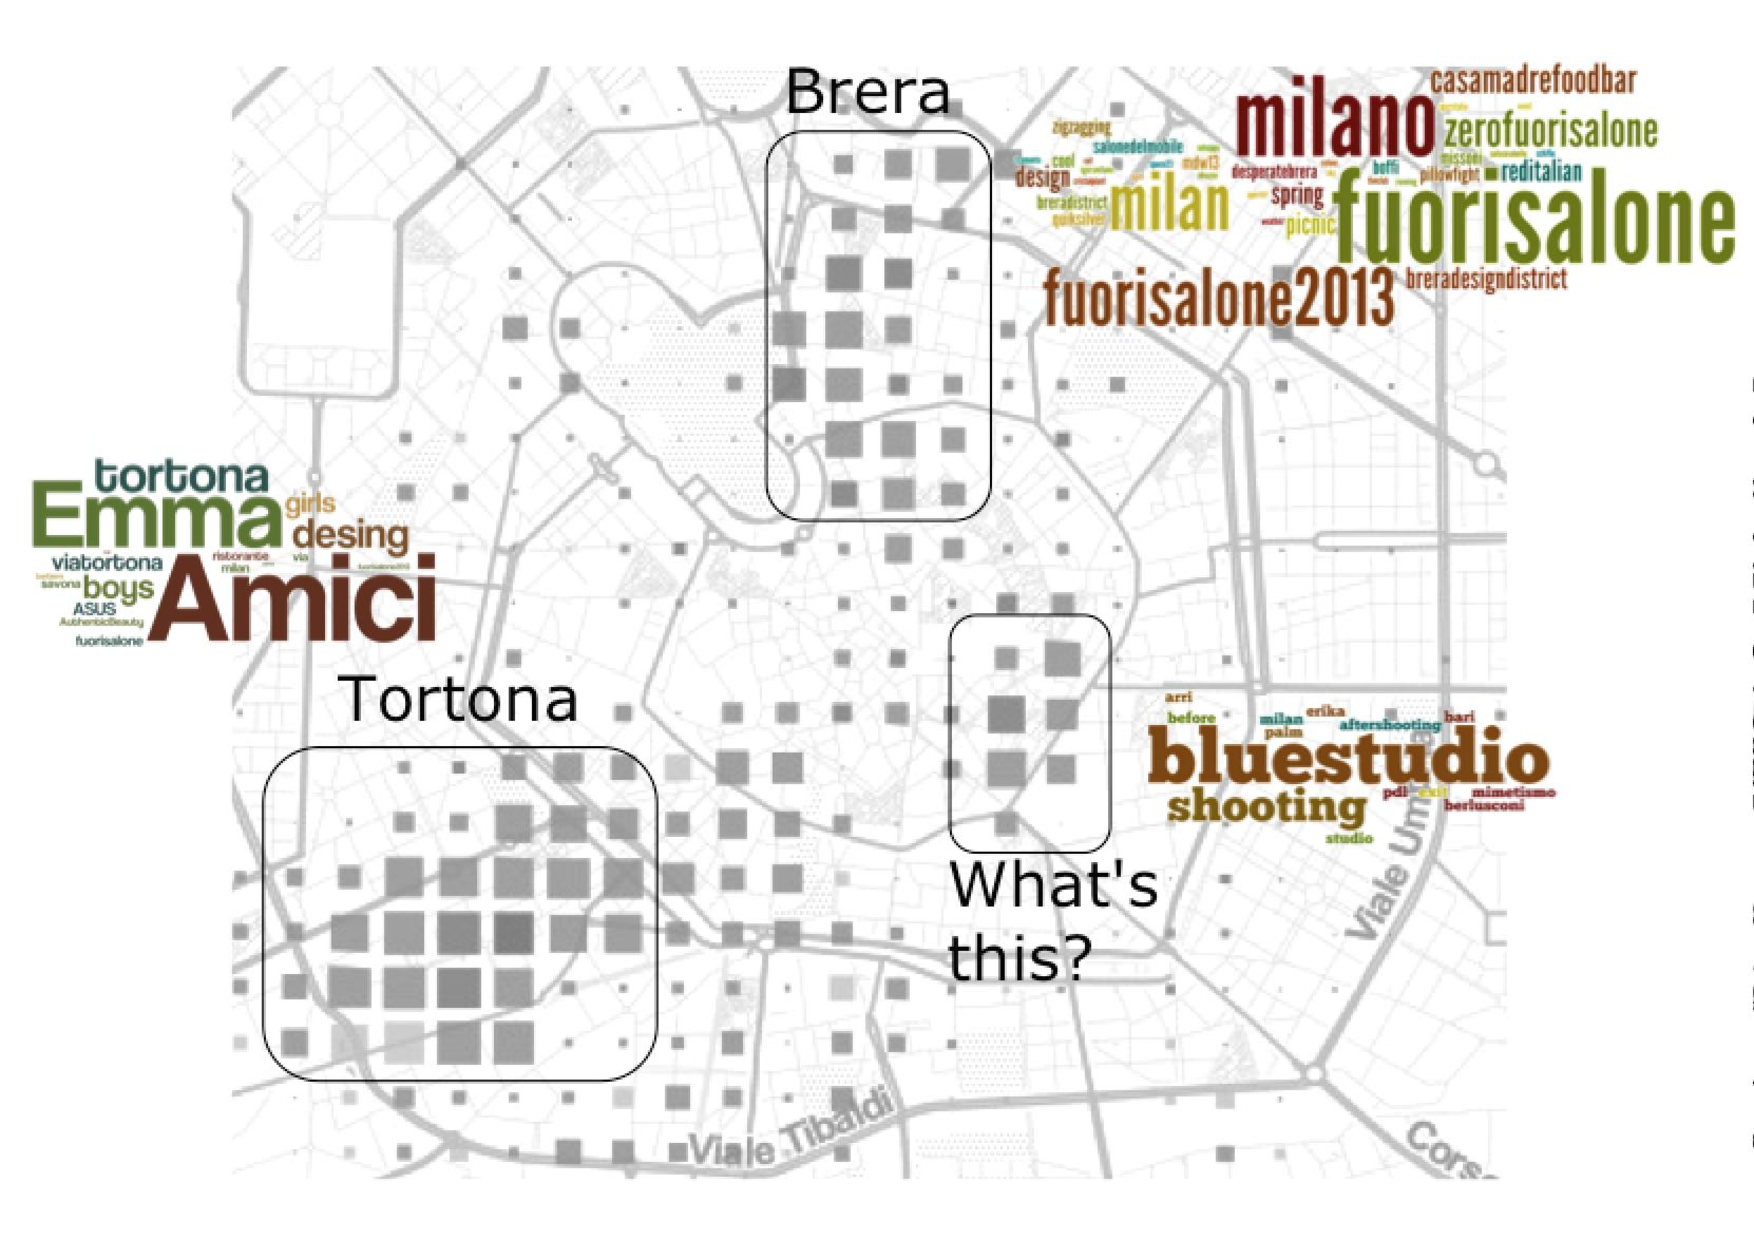
\includegraphics[width=0.49\textwidth]{img/mdw-ht-1} 
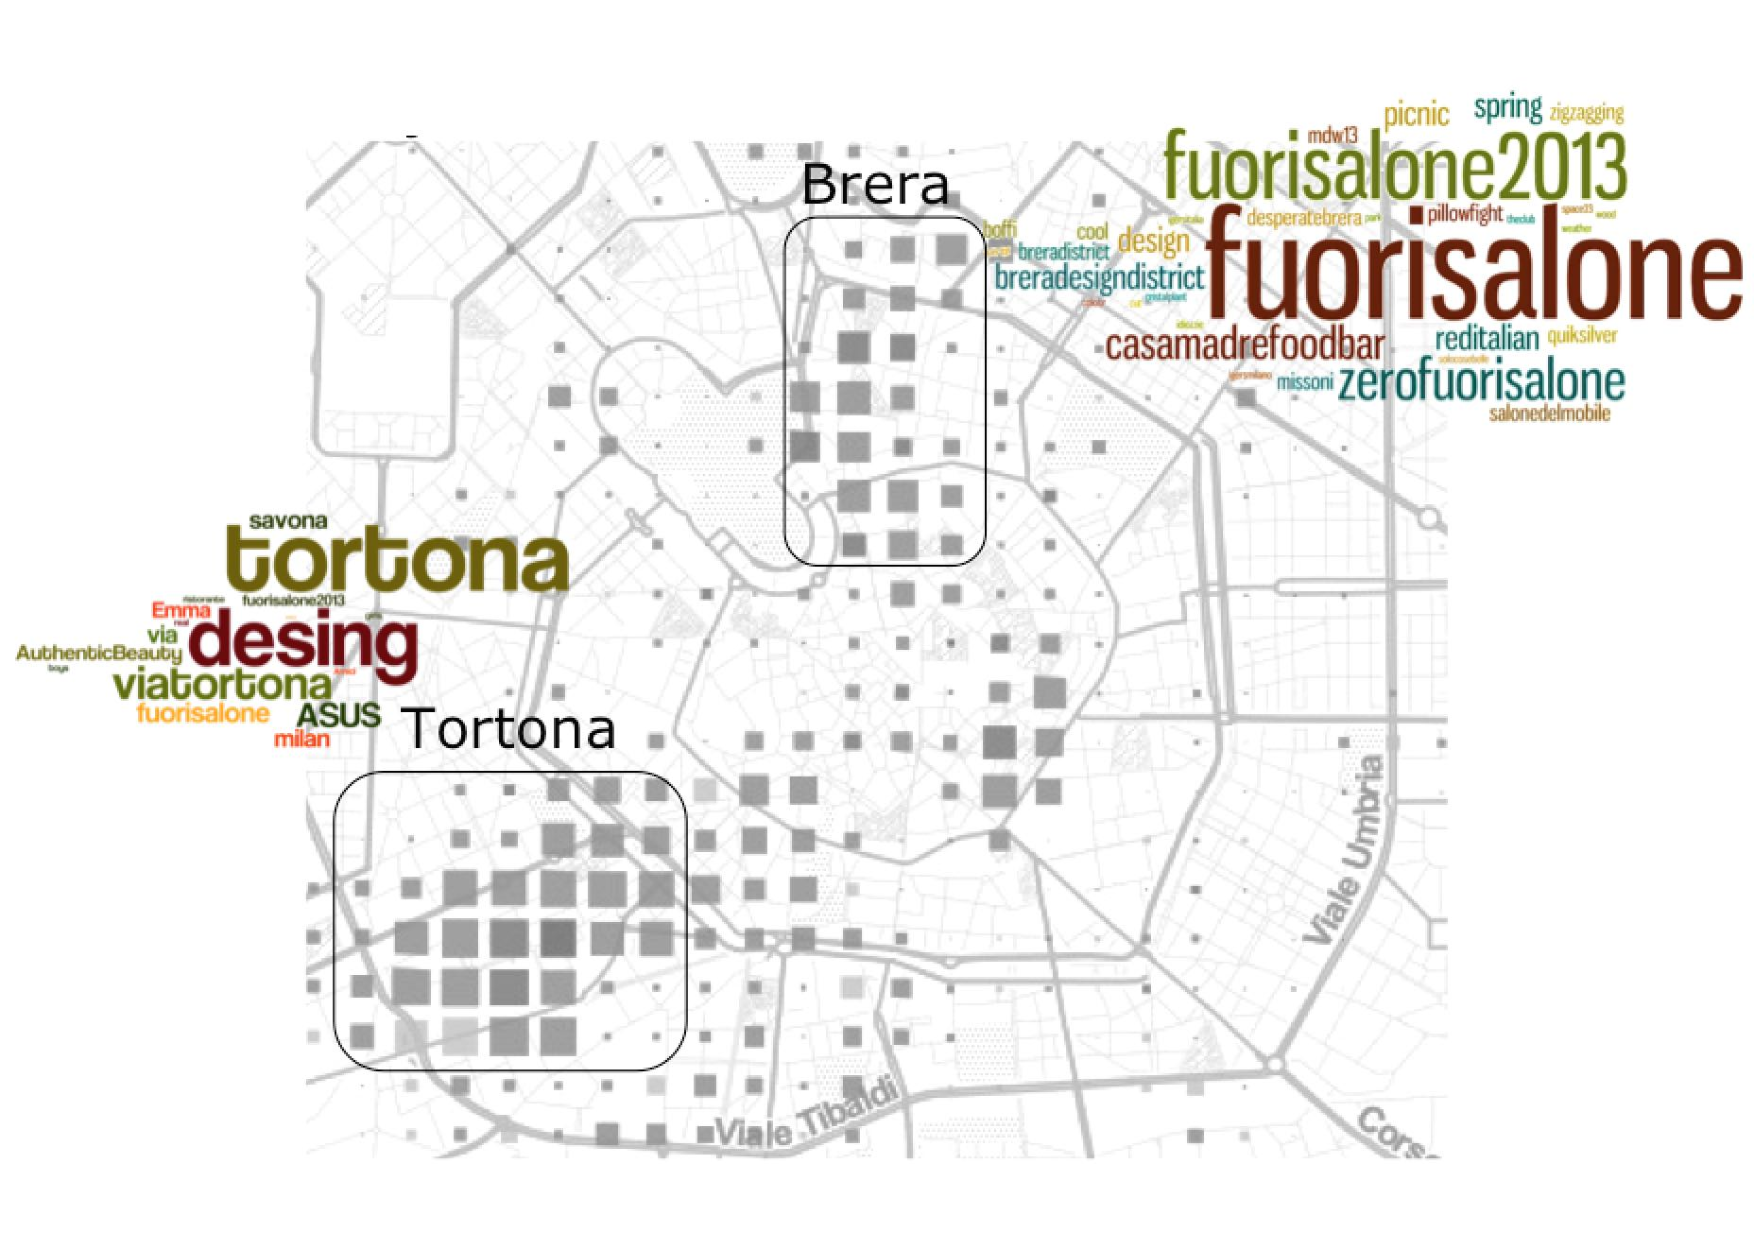
\includegraphics[width=0.49\textwidth]{img/mdw-ht-2} 
(a)\hspace{150pt} (b)
\caption{Social media used  to explain the reason of anomalous peaks of presence  in some pixels: (a) shows the most popular hashtags posted in the anomalous pixels during Milan Design Week, whereas (b) highlights the emergent hashtags, i.e., the non predicted ones. While the generic most popular tags contains also hashtag about a popular TV show (i.e., Amici or Emma), the emergent hashtags are those of Milan Design Week.}
\label{fig:de}
\end{center}
\end{figure}

As illustrated in Figure \ref{fig:de}.(a) a (partial) \textit{semantic} explanation of the mobile anomalies, can be attempted aggregating the top-10 hashtags used in those pixels. For instance, in Brera district the Italian hashtag of Milan Design Week (i.e., Fuorisalone) emerges. However, this technique is not dependable. For instance, in Tortona district also the hashtags of a popular TV show (i.e., Amici) and its protagonists (e.g., Emma) appear. Once again, the solution is in the ability to compare the current top hashtags against the those predicted by a statistical model. This allows highlighting only the emergent hashtags of this frame for the selected pixels  (see Figure~\ref{fig:de}.(b)).

\begin{figure}[t]
\begin{center}
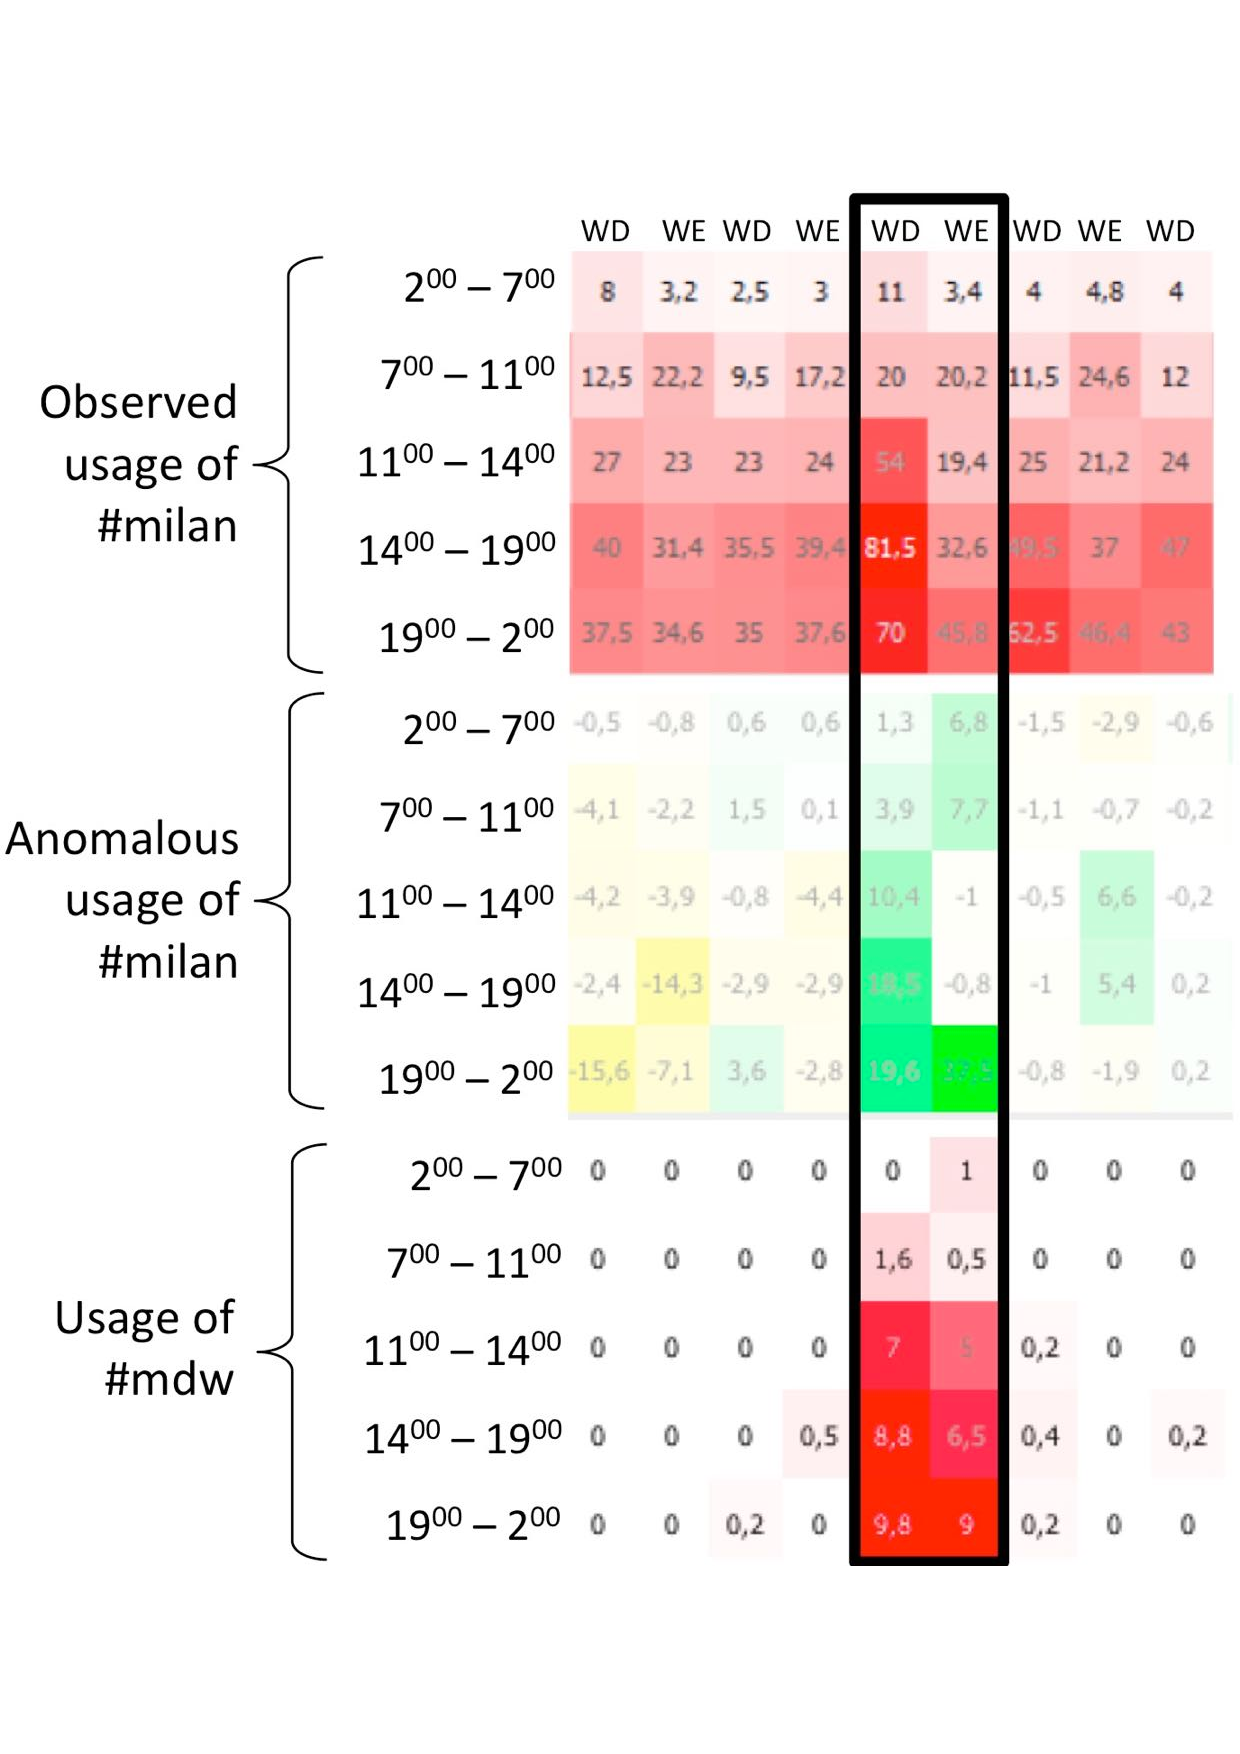
\includegraphics[width=0.5\textwidth]{img/mdw-ht-usage} 
\caption{Highlighting of anomalies in hashtag usage: The hashtag \#milan is used more often during the Milan Design Week.
Forecasting the \#milan time-series using Holt-Winter method, we were able to identify the anomalous usage, which is highly correlated to the usage of \#mdw -- the official hashtag of Milan Design Week. }
\label{fig:L}
\end{center}
\end{figure}

As one can expect, the simple Gaussian model used for the mobile activity is not appropriate to predict hashtag usage. We found, instead, that an Holt-Winter method can be used~\cite{kalekar2004time} to predict the usage over time of a specific hashtag (e.g., \#milan). In order to use Holt-Winter, we use \frappe{}: we build \textsf{SyntheticFrames} that aggregate the \textsf{CapturedFrames} in five parts of a day (i.e., 2am-7am, 7am-11am, 11am-2pm, 2pm-7pm and 7pm-2am). Moreover, as for the CDRs, we distinguish between working days and week-ends. This approach allows to build effective predictive models for hashtags about the points of interest of Milan and about popular TV shows. Figure \ref{fig:L} illustrates how this method detects the anomalous usage of \#milan during the Milan Design Week, which is highly correlated to the usage of  \#mdw -- the official hashtag of Milan Design Week.

During the Milan Design Week, using \sti{} to compare those models with the observed usage of an hashtag, we detect in real-time emerging hashtags. Figure~\ref{fig:L} illustrates how the extra usage of \#milan is correlated to the appearance of the official hashtag of Milan Design Week (i.e., \#mdw).

Using the analyses described above, CitySensing identifies pixels where people is talking about Milan Design Week. As detailed in Section~\ref{sec:cs-mdw-2013}, those pixels are not as numerous as those identified as anomalous using the CDRs. However, they match with almost absolute precision the pixels in which Milan Design Week events happen. The most interesting finding is that almost all those pixels are contained in mobile anomalous ones. This provides further experimental evidence that the anomalies observed in the CDRs are caused by the people coming to Milan for the Design Week.

The particular scheduling and geographical organization of the events of Milano Design Week, with most of the events concentrated in some specific areas of the city, enable also to perform analysis with irregular \textsf{grid}, based on the official areas of Fuorisalone.

% \begin{figure}[t]
% 	\begin{center}
% 		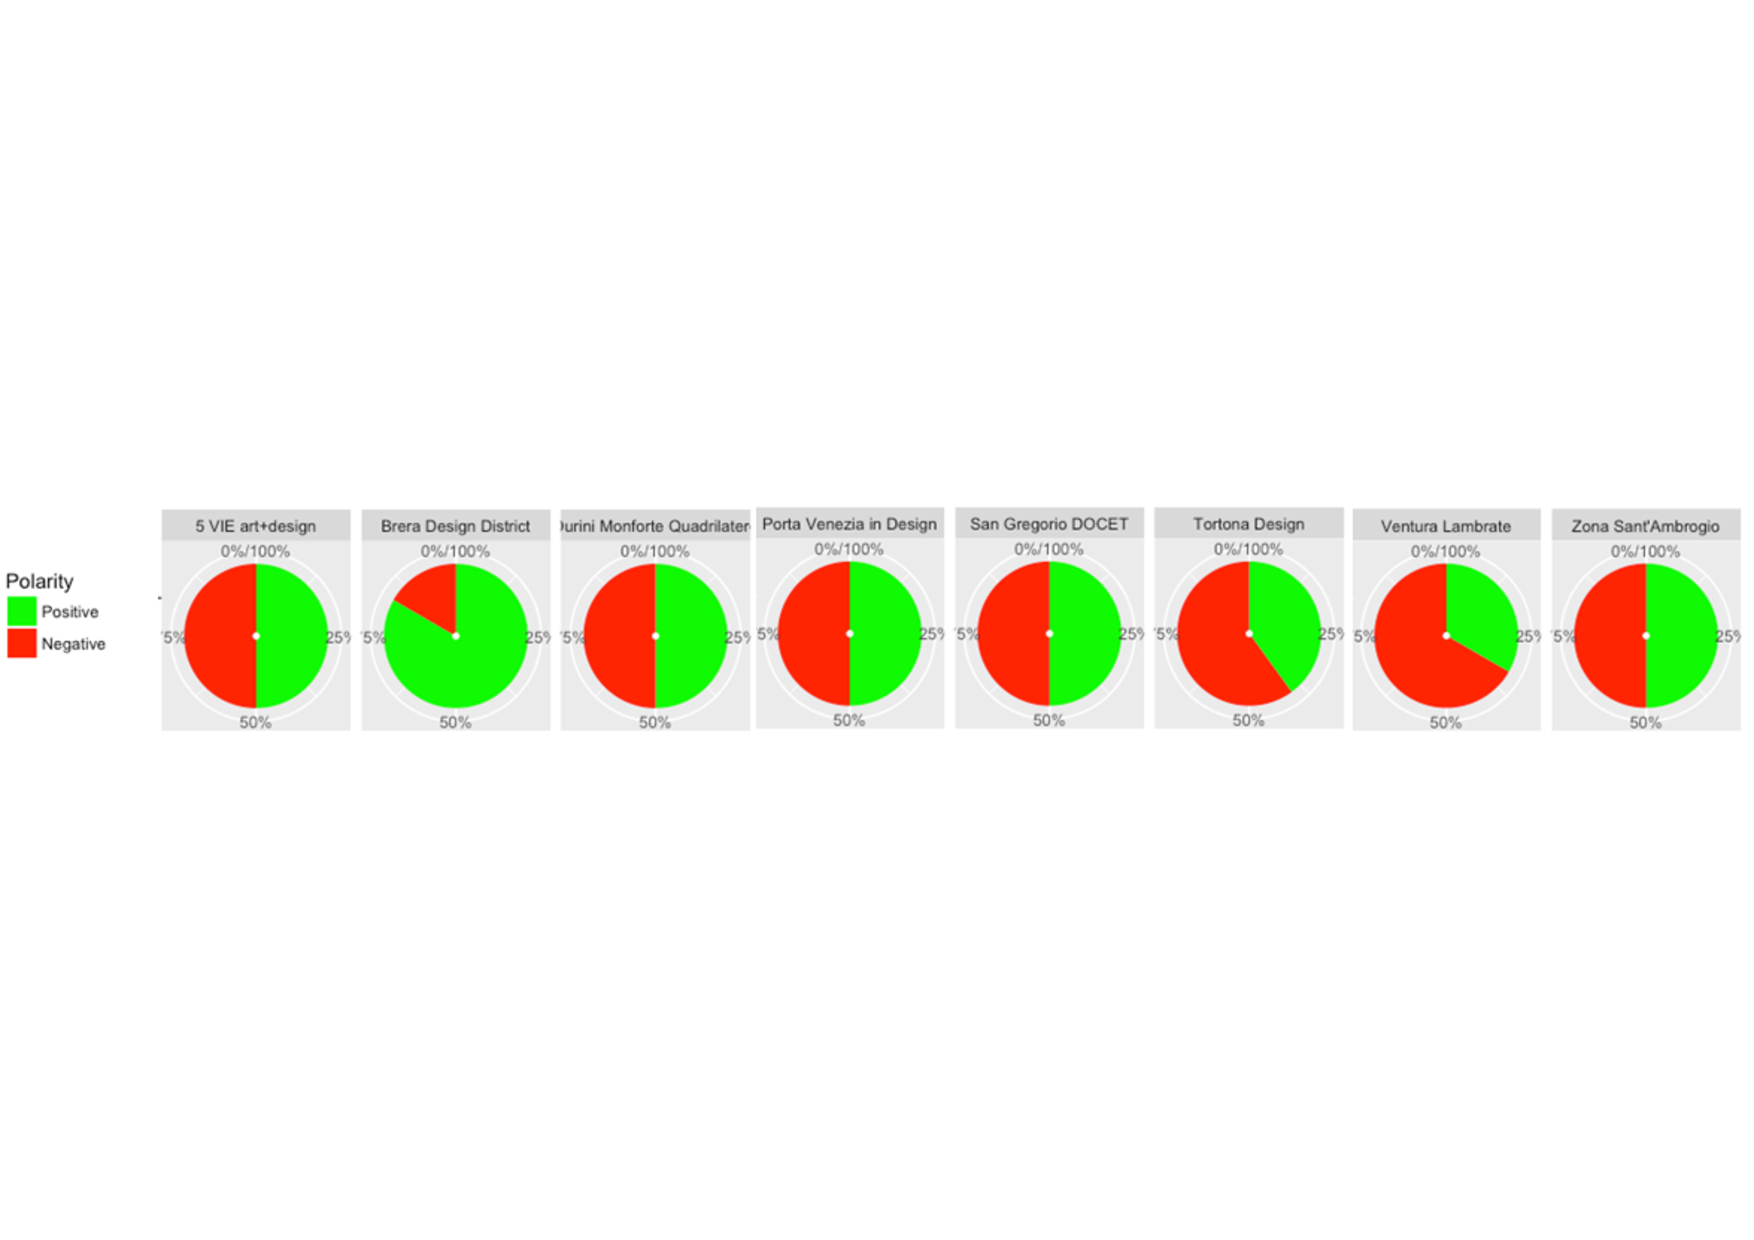
\includegraphics[width=\textwidth]{img/mdw-sentiment} 
% 		\caption{Share of positive and negative sentiment calculated for posts associated to the different MDW\ cells.}
% 		\label{fig:mdw_sentiment}
% 	\end{center}
% \end{figure}

%An examples of analysis performed on this grid is shown in Figure~\ref{fig:mdw_sentiment}, that represents the results of a semantical analysis on the text of tweets related to each area of Fuorisalone. We collect for each (irregular) \textsf{pixel} the tweets geolocated in some \textsf{place} of the \textsf{cell} and the tweets that speaks about the \textsf{event}s contained in the \textsf{pixel}, and we perform on them a semantical text analysis in order to extract the sentiment polarity of the text. Then we filtered neutral tweets and we compare the number of positive and negative tweets in each \textsf{pixel} in order to show, for each daily \textsf{frame}, which \textsf{pixel}s (that corresponds to an official area of Fuorisalone) are most successful according to the opinions of social network users.

\begin{figure}[p]
\centering
\subfloat[]{
	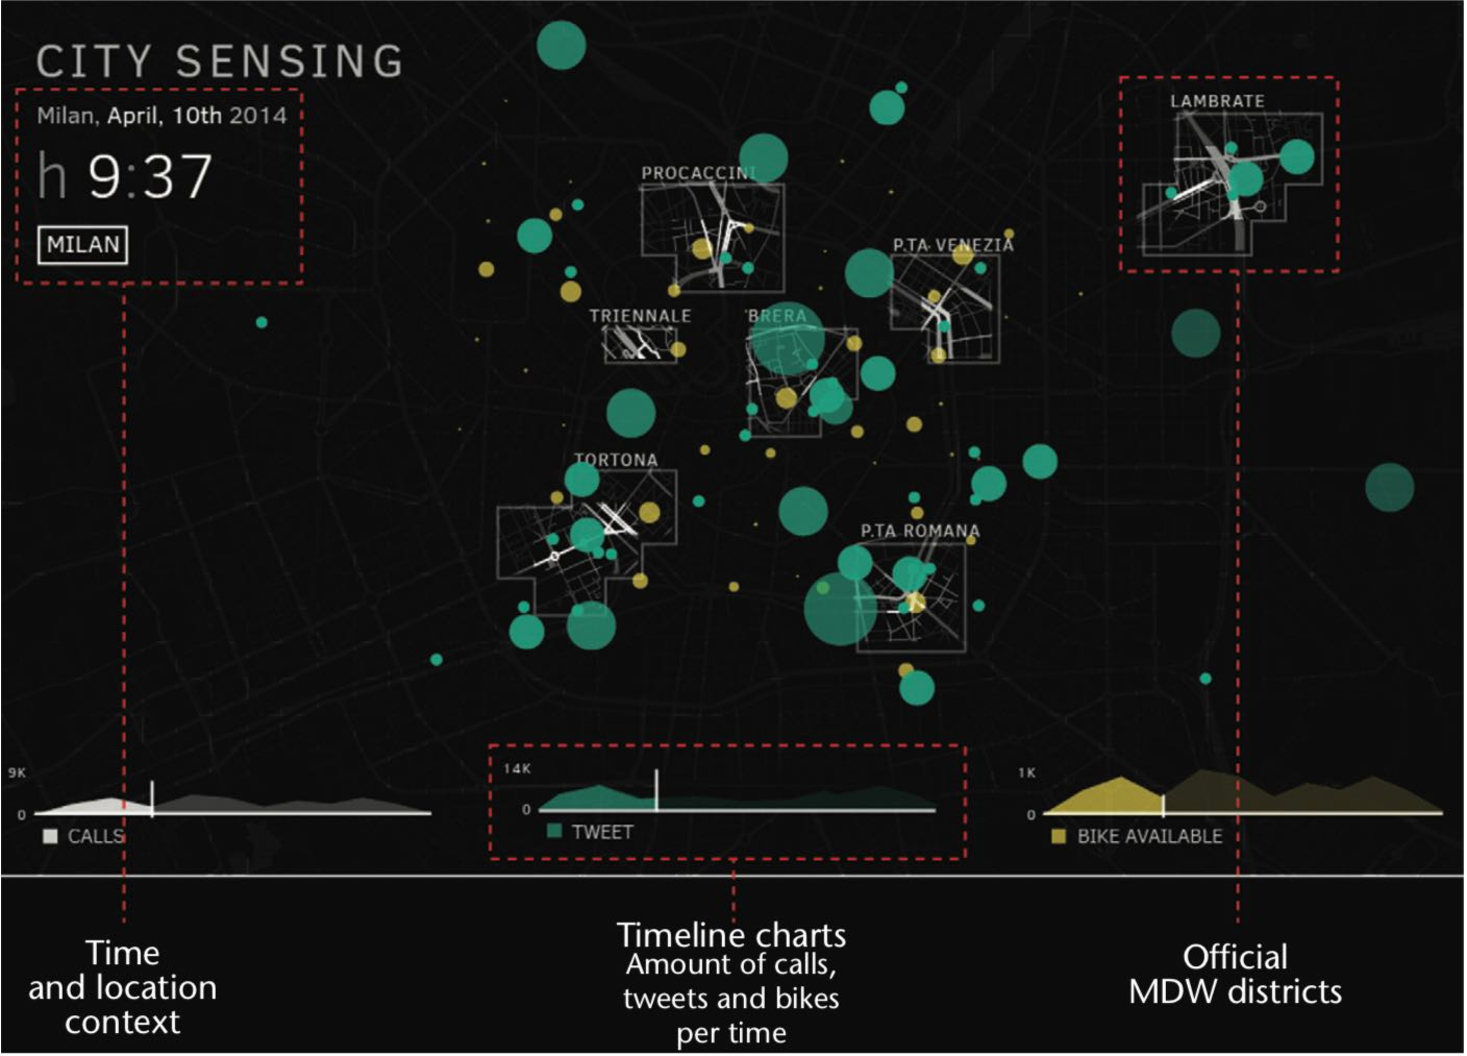
\includegraphics[width=0.52\textwidth]{img/mdw-vis-1} 
}\\
\subfloat[]{
	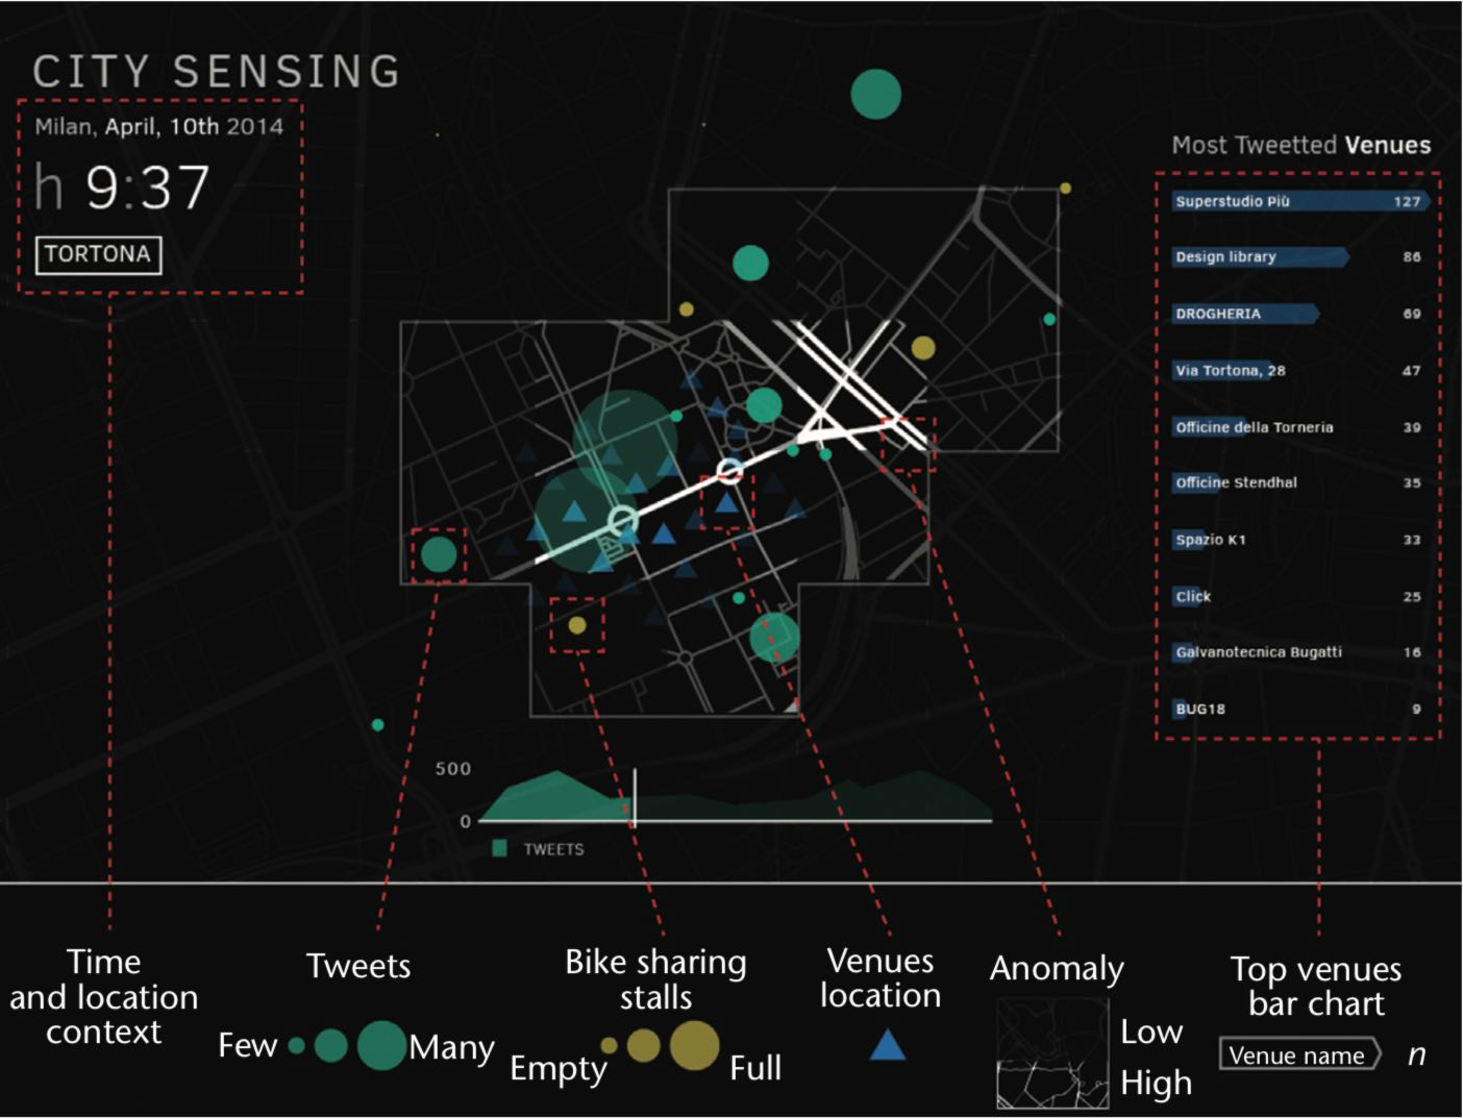
\includegraphics[width=0.52\textwidth]{img/mdw-vis-2} 
}\\
\subfloat[]{
    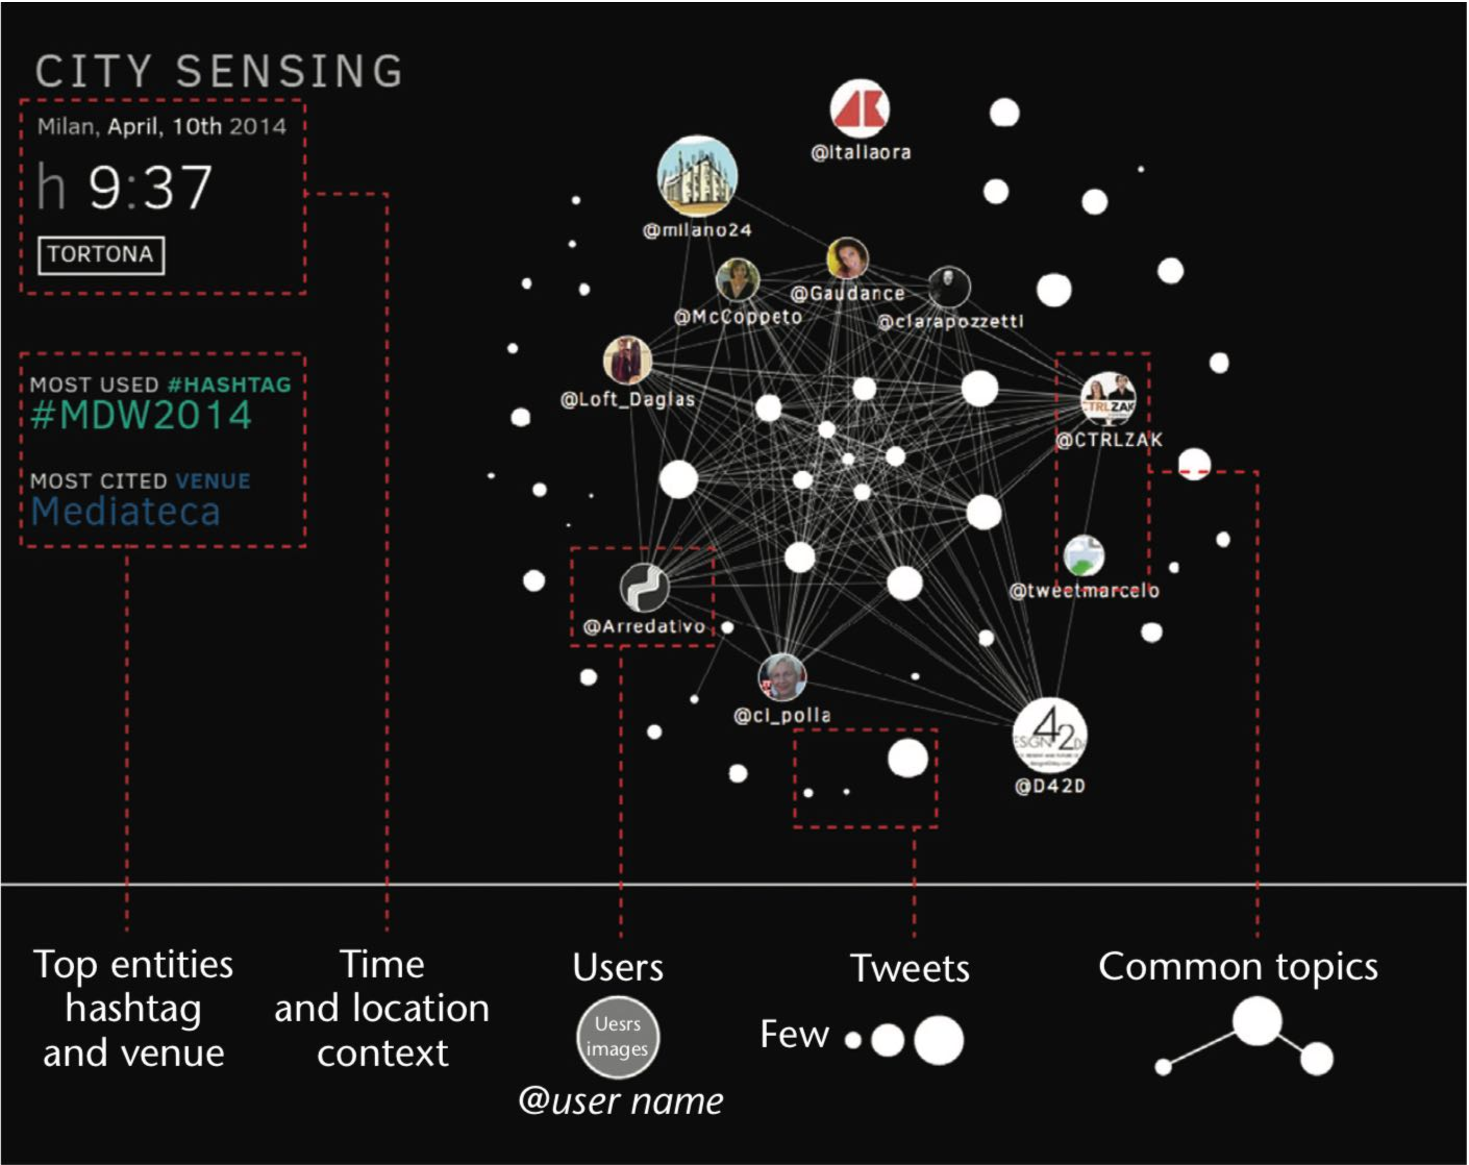
\includegraphics[width=0.52\textwidth]{img/mdw-vis-3} 
}
\caption{MDW2014 CitySensing installation geographical view (a) at city level, where the visualization highlights the pixels of official MDW districts, and (b) at district level, the map is zoomed and centered on the district. (c) The graph view displays the evolution of the graph of people visiting MDW2014 places and events. (source~\cite{DBLP:journals/ieeemm/BalduiniVALAC15}).}
\label{fig:mdw-2014-vis}
\end{figure}

% \begin{figure}[t]
%   \begin{minipage}{.33\textwidth}
%       \centering
%       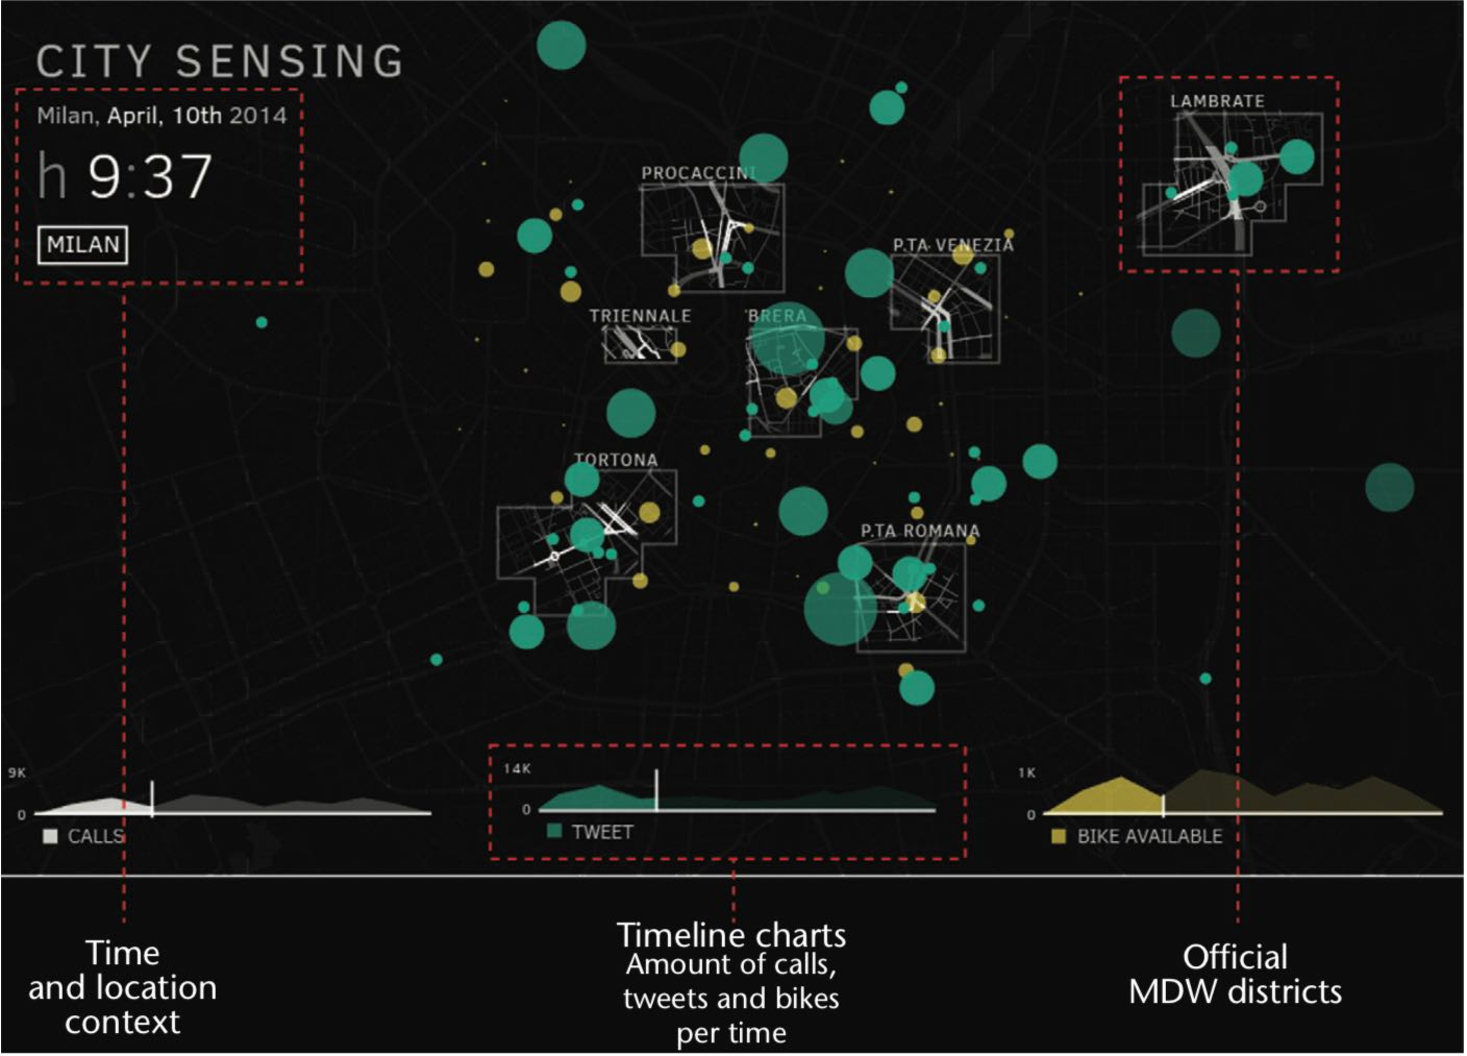
\includegraphics[width=0.3\linewidth]{img/mdw-vis-1}
%   \end{minipage}
%   \begin{minipage}{0.33\textwidth}
%       \centering
%       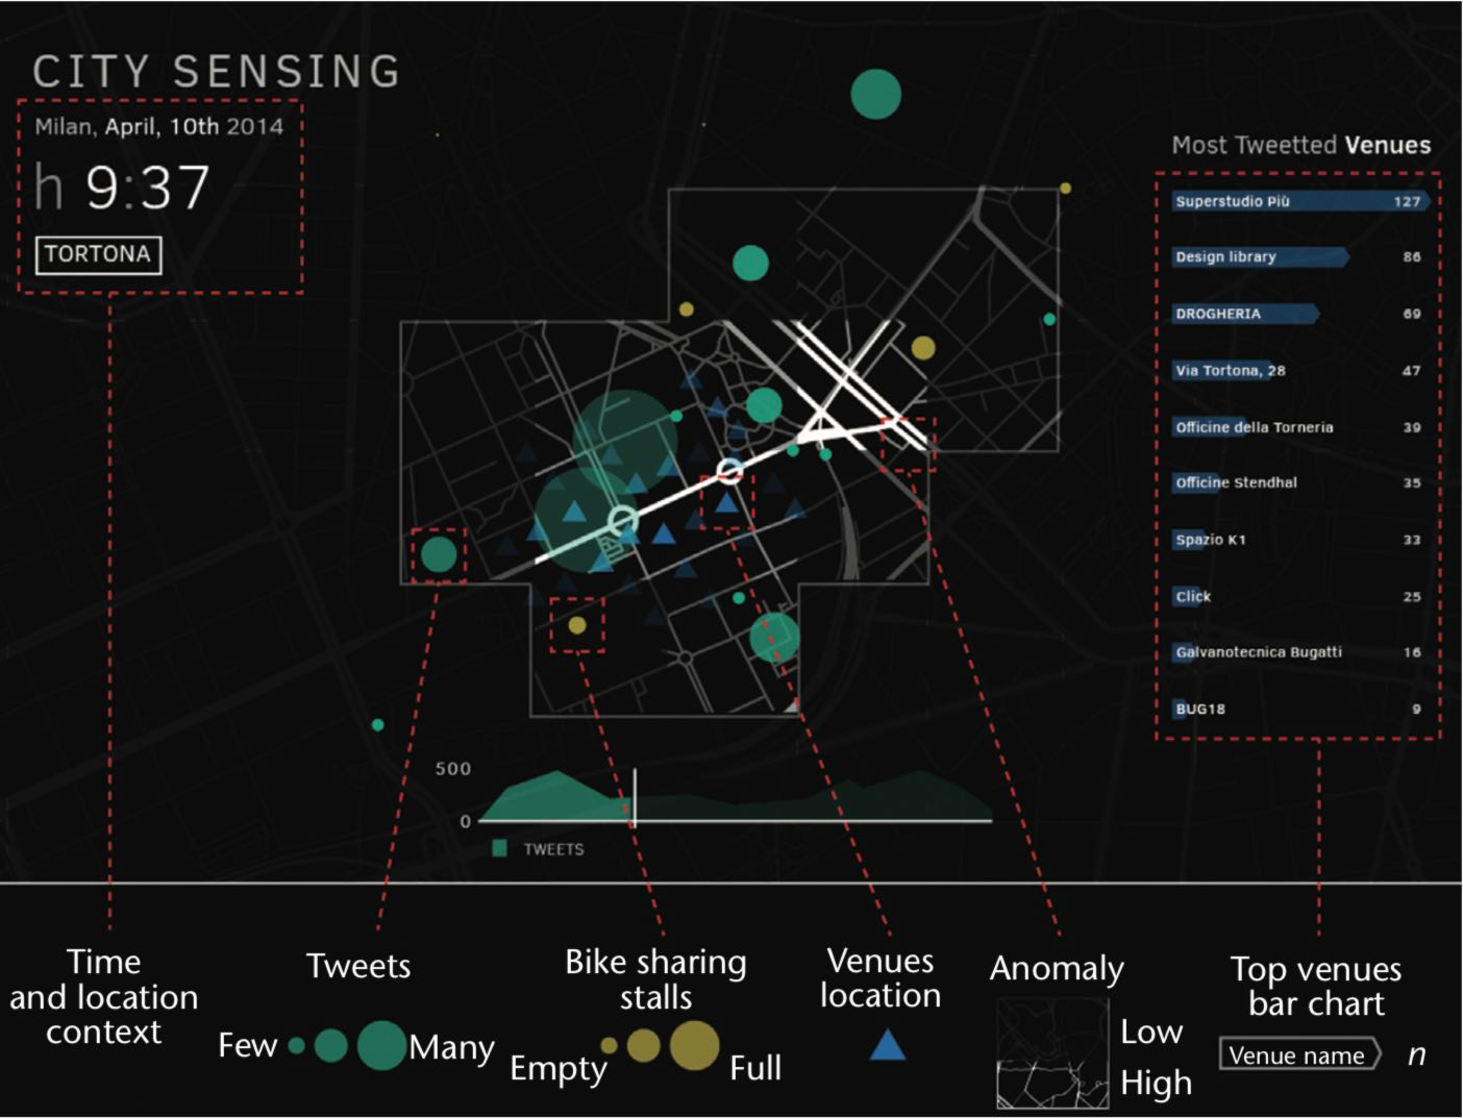
\includegraphics[width=0.3\linewidth]{img/mdw-vis-2} 
%   \end{minipage}
%   \begin{minipage}{0.33\textwidth}
%       \centering
%       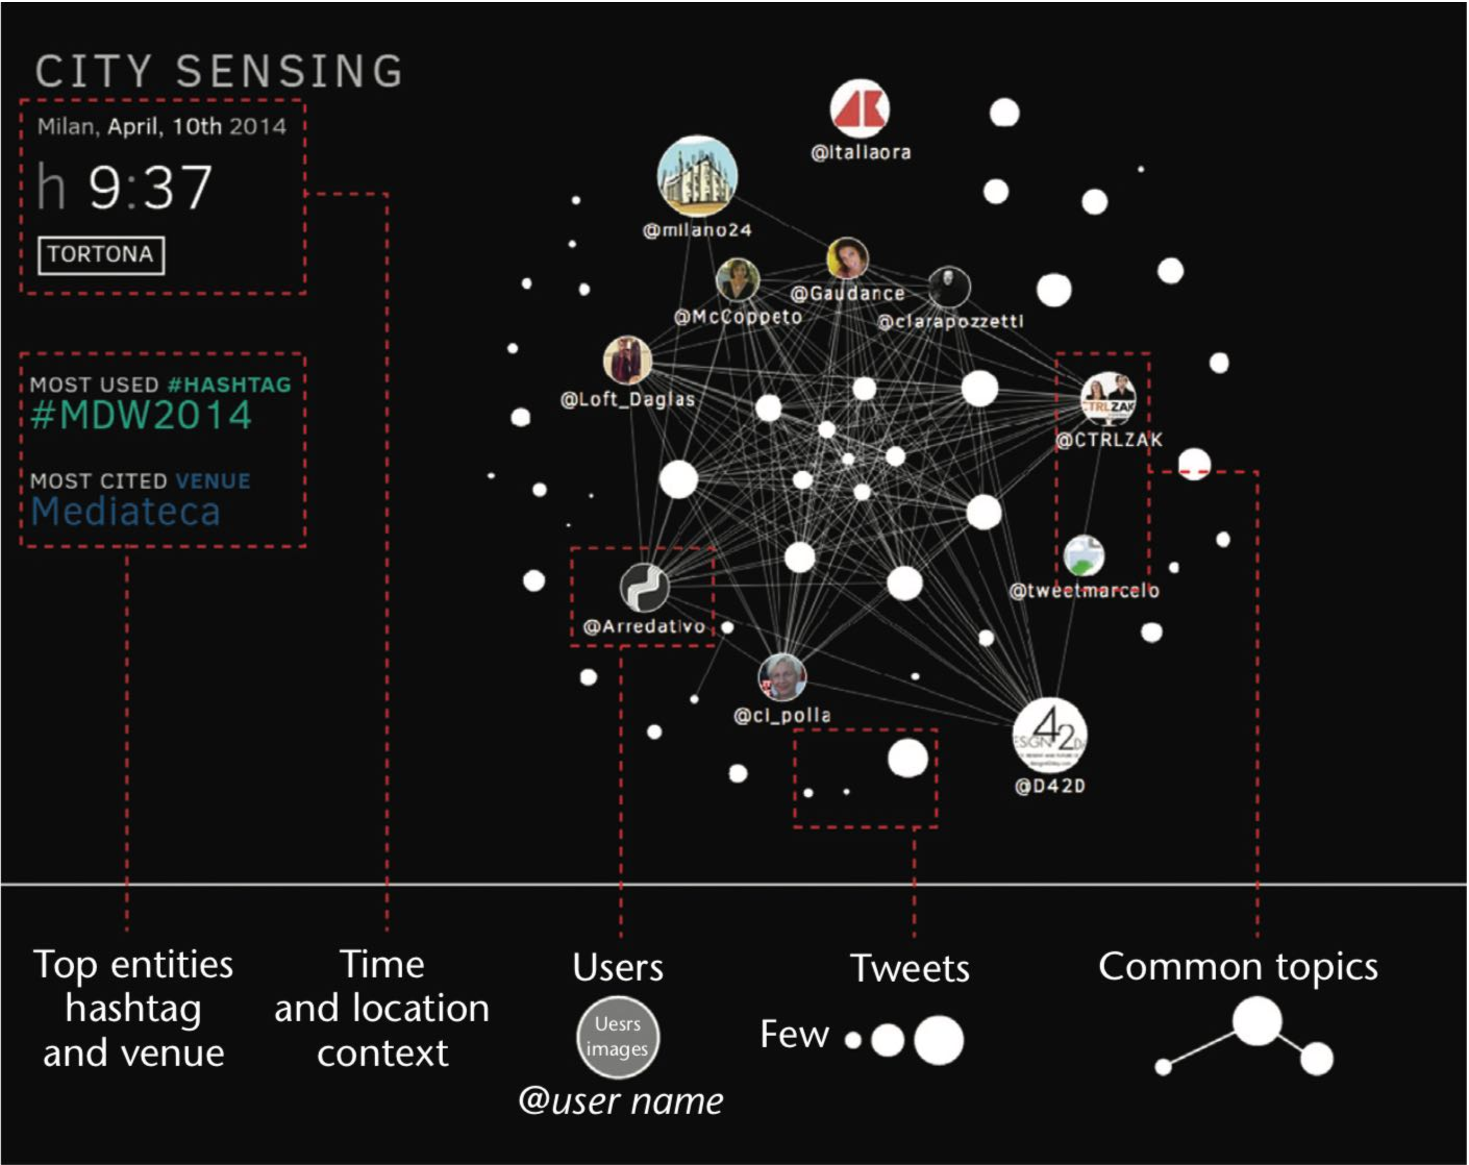
\includegraphics[width=0.3\linewidth]{img/mdw-vis-3} 
%   \end{minipage}
%   \caption{(a) MDW2014 CitySensing installation geographical view (a) at city level, where the visualization highlights the pixels of official MDW districts, and (b) at district level, the map is zoomed and centered on the district. (c) The graph view displays the evolution of the graph of people visiting MDW2014 places and events. (source~\cite{DBLP:journals/ieeemm/BalduiniVALAC15}).}
%   \label{fig:mdw-2014-vis}
% \end{figure}

% \begin{figure}[!t]
% \centering
% \minipage{\textwidth}
%   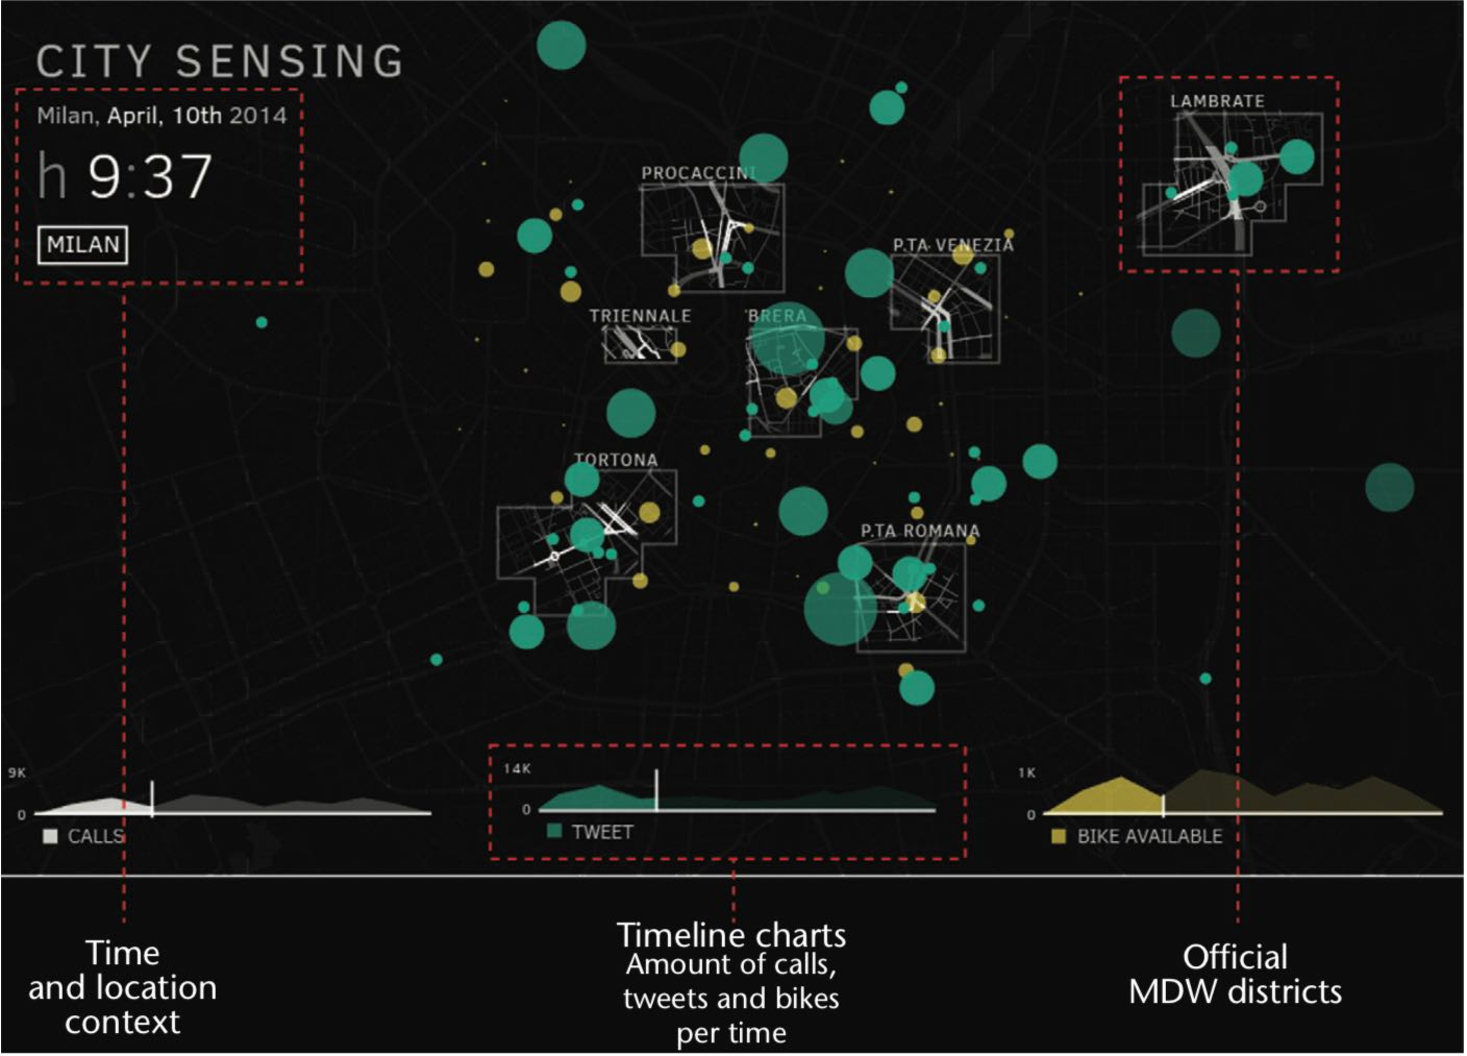
\includegraphics[width=0.5\linewidth]{img/mdw-vis-1}
% \endminipage\hfill \\
% \minipage{\textwidth}
%   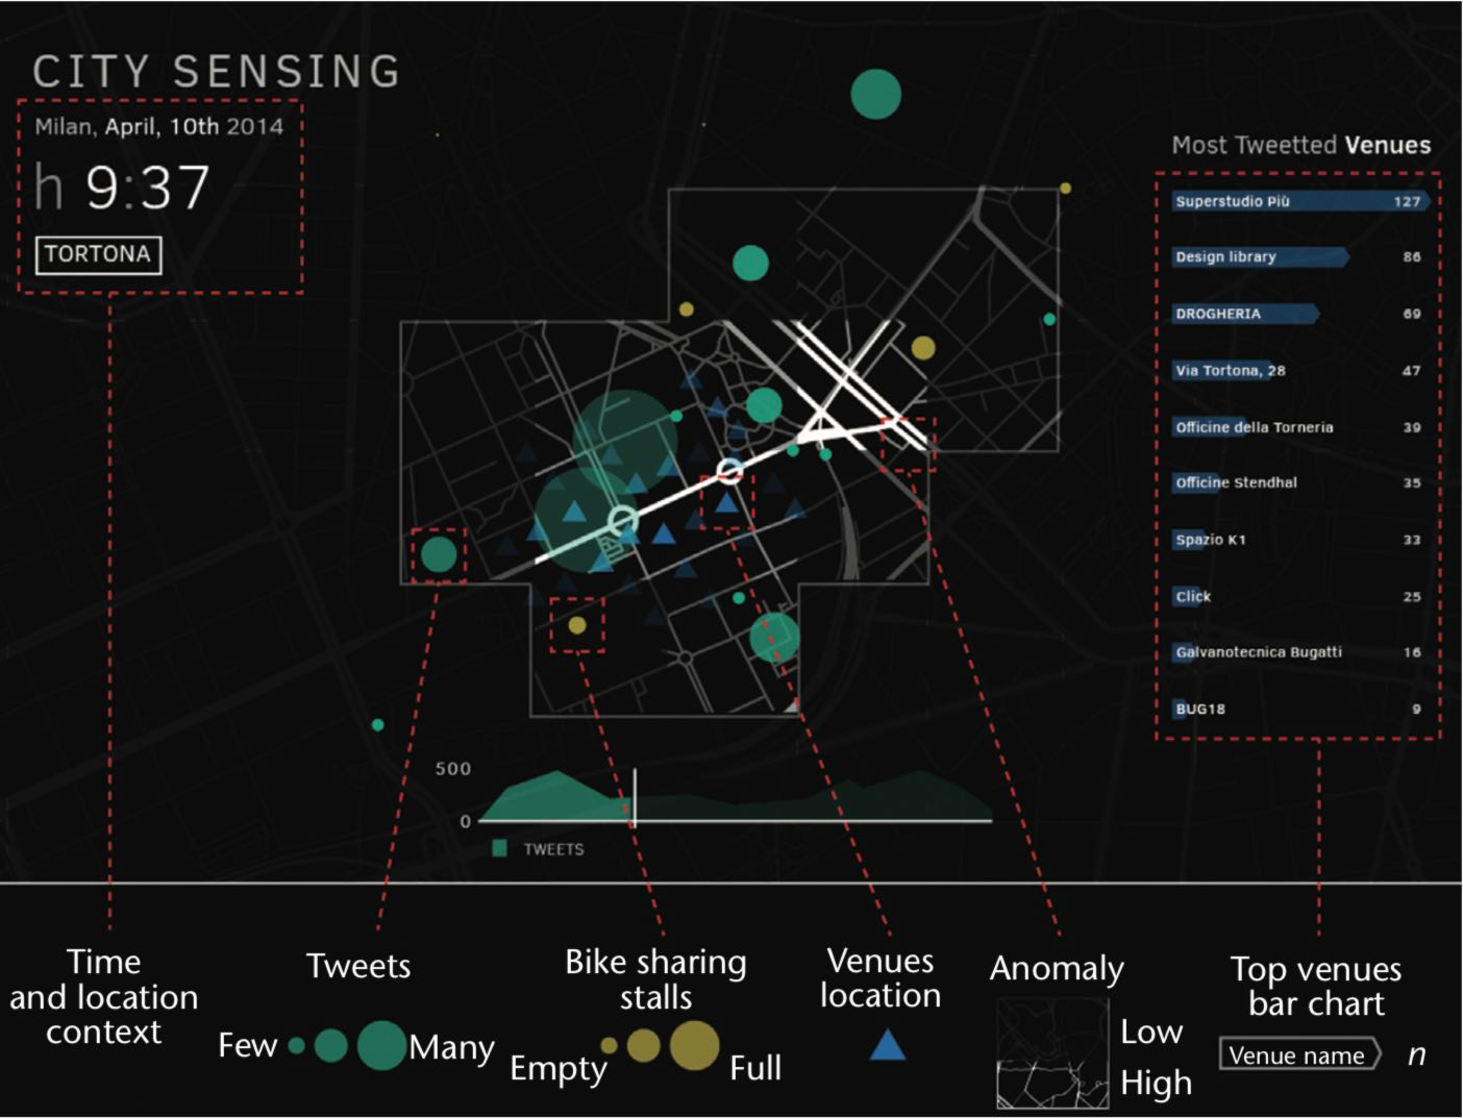
\includegraphics[width=0.5\linewidth]{img/mdw-vis-2}
% \endminipage\hfill \\
% \minipage{\textwidth}
%   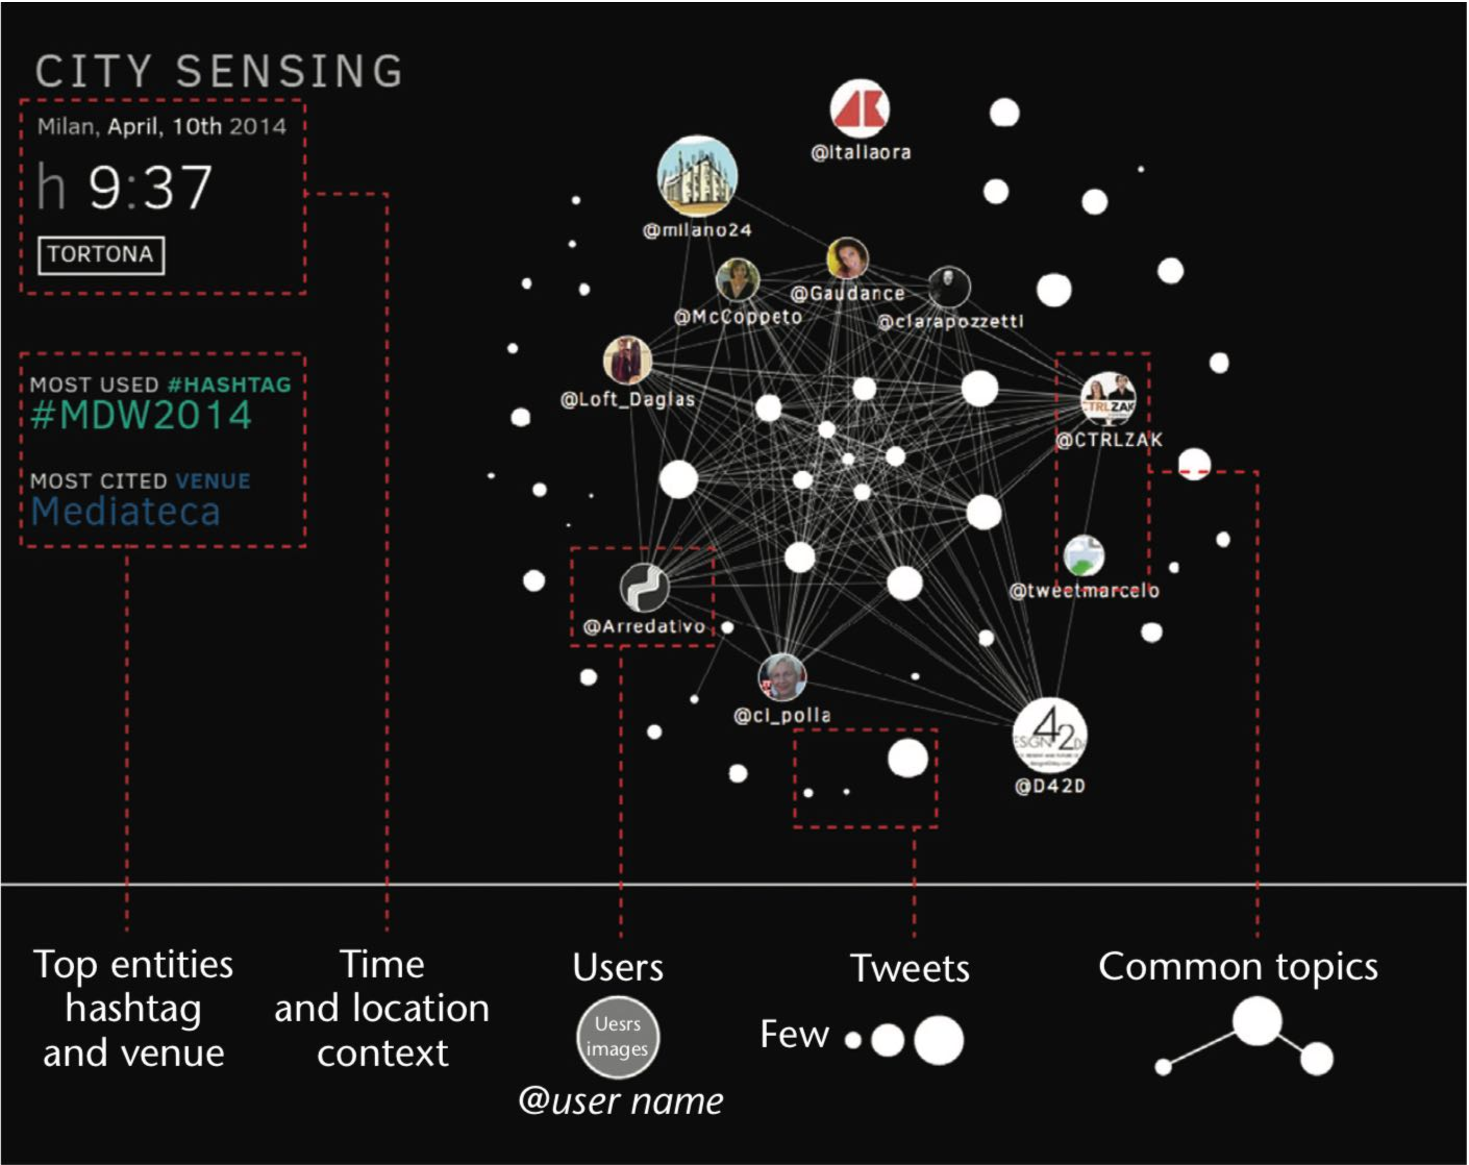
\includegraphics[width=0.5\linewidth]{img/mdw-vis-3}
% \endminipage
%  \caption{(a) MDW2014 CitySensing installation geographical view (a) at city level, where the visualization highlights the pixels of official MDW districts, and (b) at district level, the map is zoomed and centered on the district. (c) The graph view displays the evolution of the graph of people visiting MDW2014 places and events. (source~\cite{DBLP:journals/ieeemm/BalduiniVALAC15}).}
%  \label{fig:mdw-2014-vis}
% \end{figure}

The CitySensing visualizations exploit the \frappe{} concepts to relate time and space.
They comprise two main views: a geographical view (see Figures~\ref{fig:mdw-2014-vis}(a) and \ref{fig:mdw-2014-vis}(b)) that displays signals on a static map of Milan, and a graph view (see Figure~\ref{fig:mdw-2014-vis}(c)) that displays the evolution of the graph of people visiting MDW2014 places and events. Both can be zoomed in at the city or district level. The system underpinning the views enables the story to be told in nearly real time, but the visualized phenomenon is better viewed quickly, with the system playing a day in few minutes. To this end, a new frame, which aggregates 15 minutes of data, is displayed every 2 seconds\footnote{\url{http://citysensing.fuorisalone.it}, \url{http:// youtu.be/MOBie09NHxM}}.

Finally, we perform an empirical evaluation of \frappe{} in order to understand how the CitySensing visualizations ease the attendees' understanding of data dynamics and, consequently, validate the \textsf{Hp.3}. 

\begin{figure}[p]
\centering
\subfloat[]{
        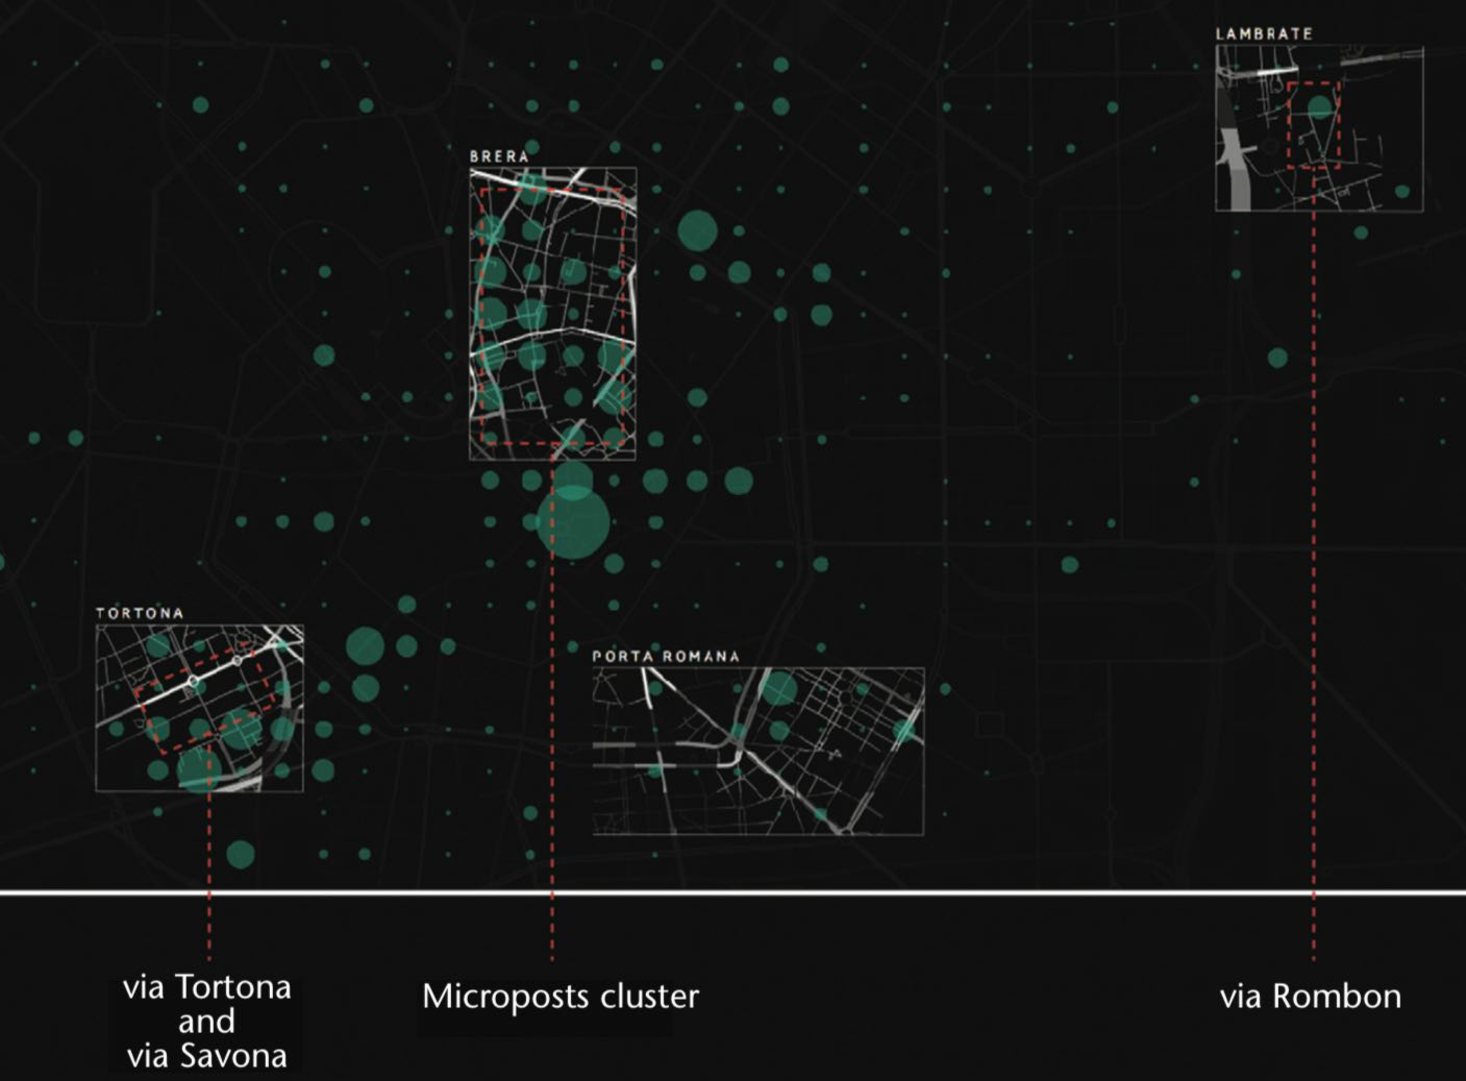
\includegraphics[width=.63\linewidth]{img/mdw-vis-4}
}\\
\subfloat[]{
        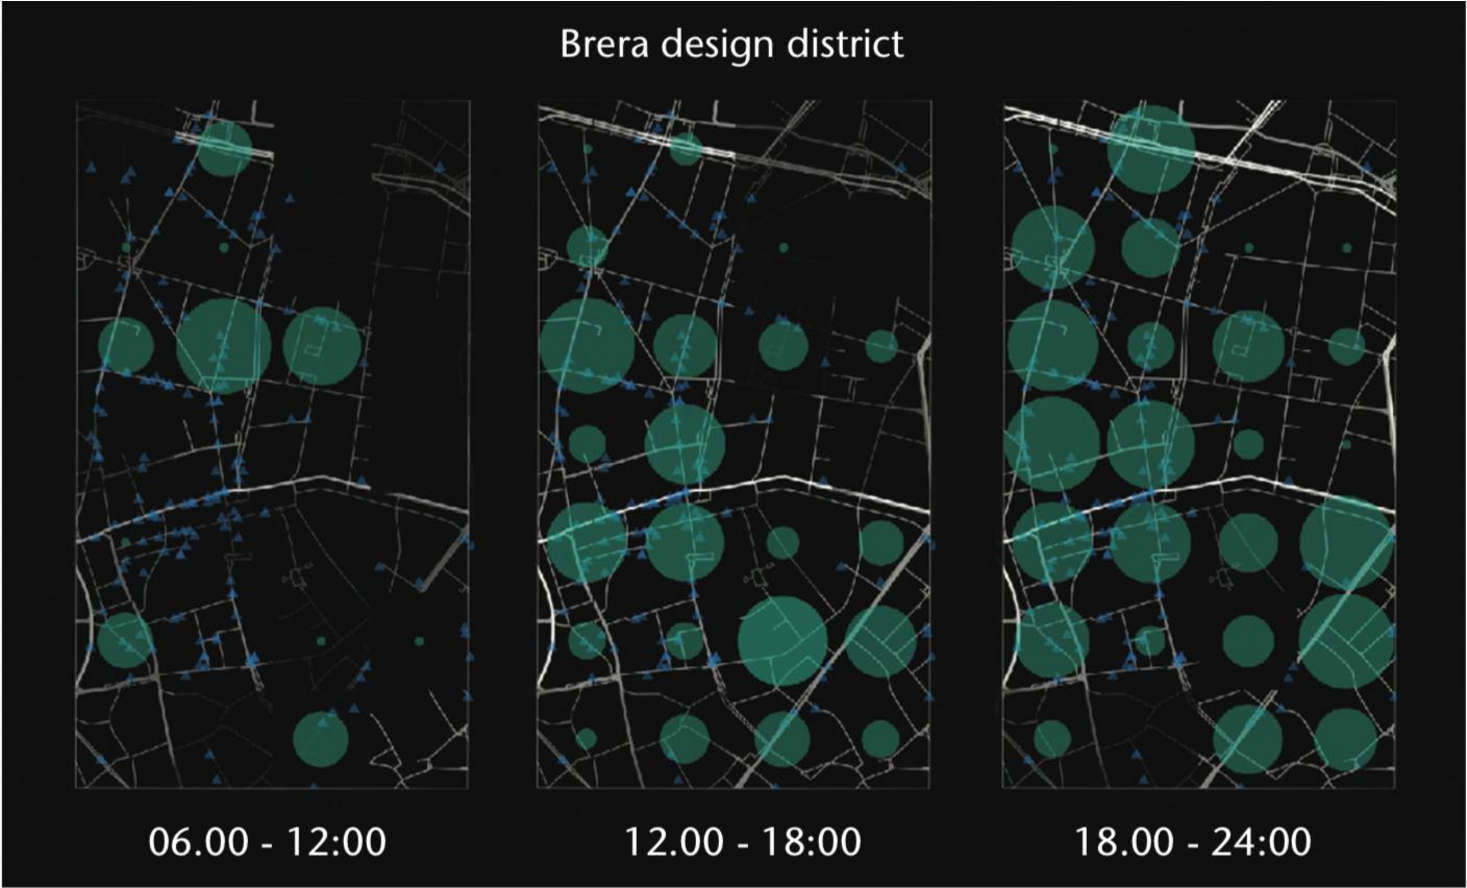
\includegraphics[width=.63\linewidth]{img/mdw-vis-5}
}\\
\subfloat[]{
        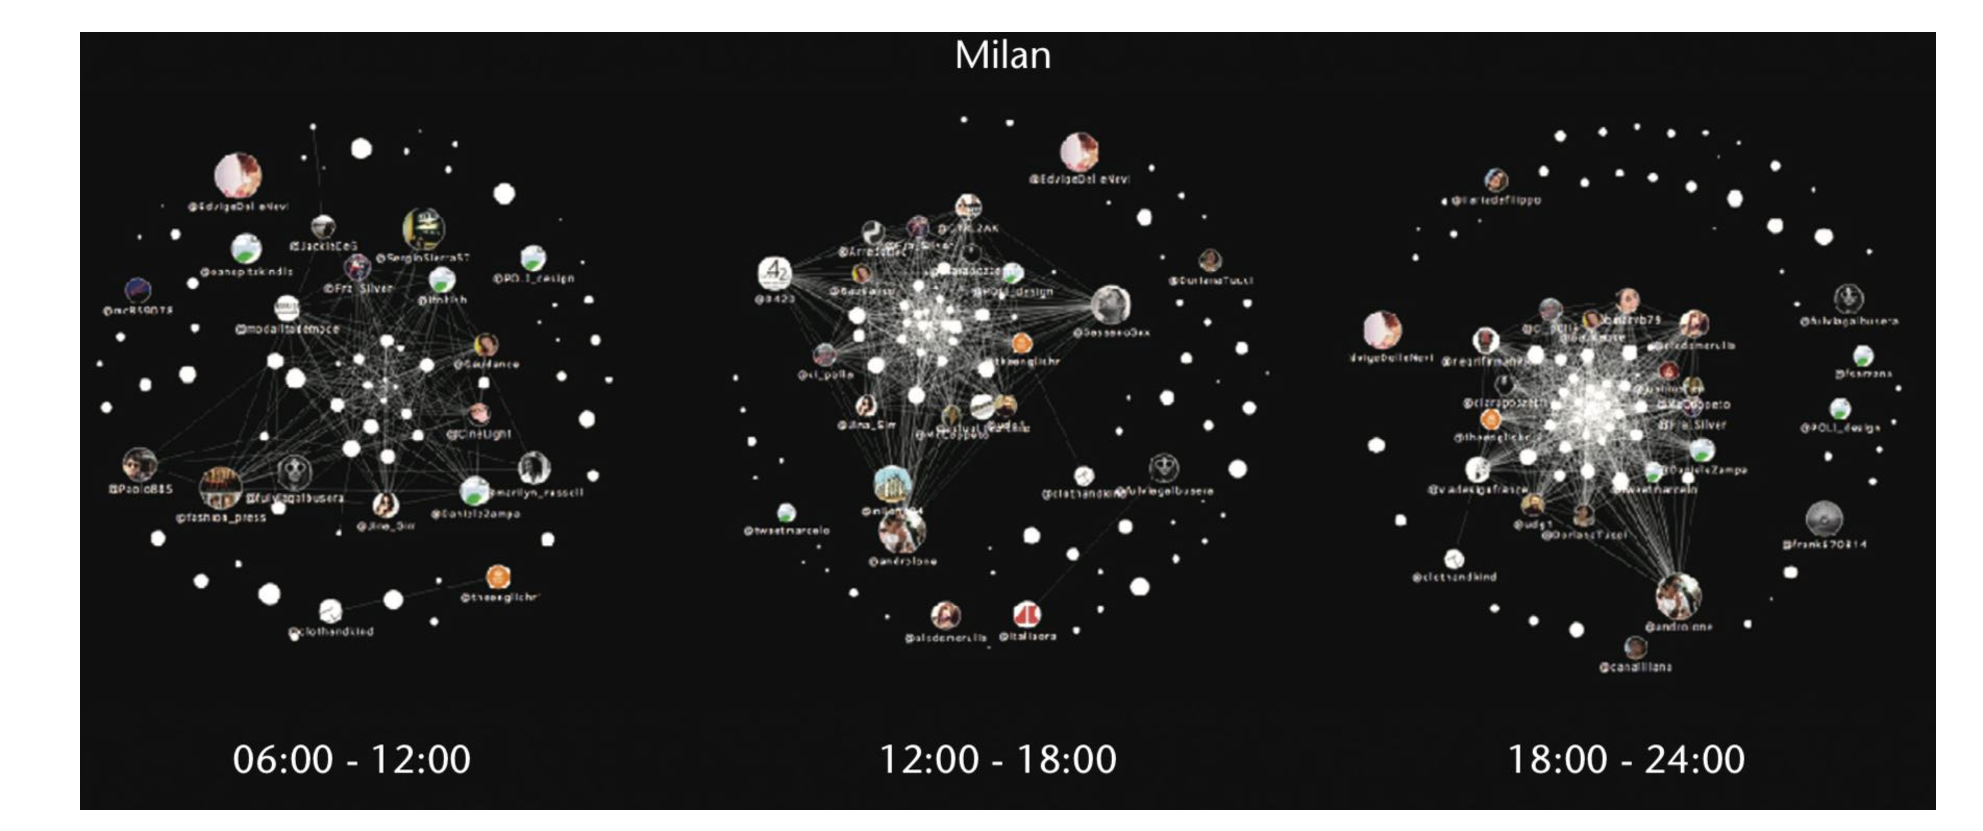
\includegraphics[width=.63\linewidth]{img/mdw-vis-6}
}
\caption{(a) The correlation between the social and mobile anomaly signals is readable in the story told by the geographical view at city level. On 10 April 2014, the social and mobile anomaly signals tell the success of MDW districts: Brera and Tortona beat all others. (b) A geographical view in which the social and mobile anomaly signals tell the daily pattern of activity in Brera. (c) This graph view highlights the scale-free nature of the graph of people when connected by the places, events, and hashtags they discuss on social media. (source~\cite{DBLP:journals/ieeemm/BalduiniVALAC15}).}
\label{fig:eval-empirical}
\end{figure}

We start from the author-driven perspective, illustrating the visualizations as the people who watched the installation in Mediateca Santa Teresa experienced them. Then, we take the reader-driven perspective and report on the results of a questionnaire meant to assess whether the audience could guess the visualizations' intended message.

Figure~\ref{fig:eval-empirical}(a) illustrates how the correlation between the social and mobile anomaly signals is readable in the story told by the geographical view at the city level. The figure represents a cumulative view of the frames between 6:00 and 24:00 on 10 April (the most active day in 2014). The majority of the streets of MDW districts "spot out" that is, the pixel highlighted by the mobile anomaly signal are MDW places. Furthermore, a clear pattern emerges: the MDW social signal (the green circles) originates from MDW districts.

Figure~\ref{fig:eval-empirical}(b) presents the geographical view, but it focuses on the Brera district. This view illustrates the evolution of the social and mobile anomaly signals over three frame groups (06:00--12:00, 12:00--18:00, and 18:00--24:00) on 10 April 2014. The places where MDW events are held normally open in the late morning, but the majority of the events start in the afternoon. This is clearly visible both in the value of the mobile anomaly signal (mapped to the opacity of the pixels) and the volume of the social signal (mapped in the size of the green circles): both signals increase in most of the pixels and especially in those containing MDW places (blue triangles).

Figure~\ref{fig:eval-empirical}(c) illustrates the graph view. It shows the evolution of the same three frame groups on 10 April 2014. During the morning, few users are linked by topics related to MDW; in the afternoon, a cluster of people talking about places and events of MDW appears; and in the evening, just few users remain unlinked. This is a direct consequence of the long-tail distribution of the discussion topics: 80 percent of the users talk about 20 percent of the places/events, while the remaining 20 percent of the users talk about the other 80 percent of places/events.

This pattern repeats over the days at city scale and in the Brera and Tortona districts. It disappears when MDW ends.
To verify the \textsf{Hp.3}, we asked people without specific skills in data visualization and analytics to guess the message of the views shown in Figure~\ref{fig:eval-empirical}(a)~and~\ref{fig:eval-empirical}~(c). We asked them the six questions reported in Figure~\ref{fig:eval-empirical-quest}. In four cases, we asked true-or-false questions, and in two cases, we asked questions that had no correct answer (see "uncertain" in the figure). The correct answers are underlined in Figure~\ref{fig:eval-empirical-quest}. As the distribution of the answers of the 23 responders shows, the messages we intended to transmit were correctly guessed. The responders correctly correlated the social and the mobile anomaly signals when the correlation was not evident and could not guess the correct answer when the correlation was not present. The same happens when they guess the meaning of the graph that links people based on the places and events that they jointly discussed.
Those results validate Hypothesis~\textsf{Hp.3}.

\begin{figure}[t]
\centering
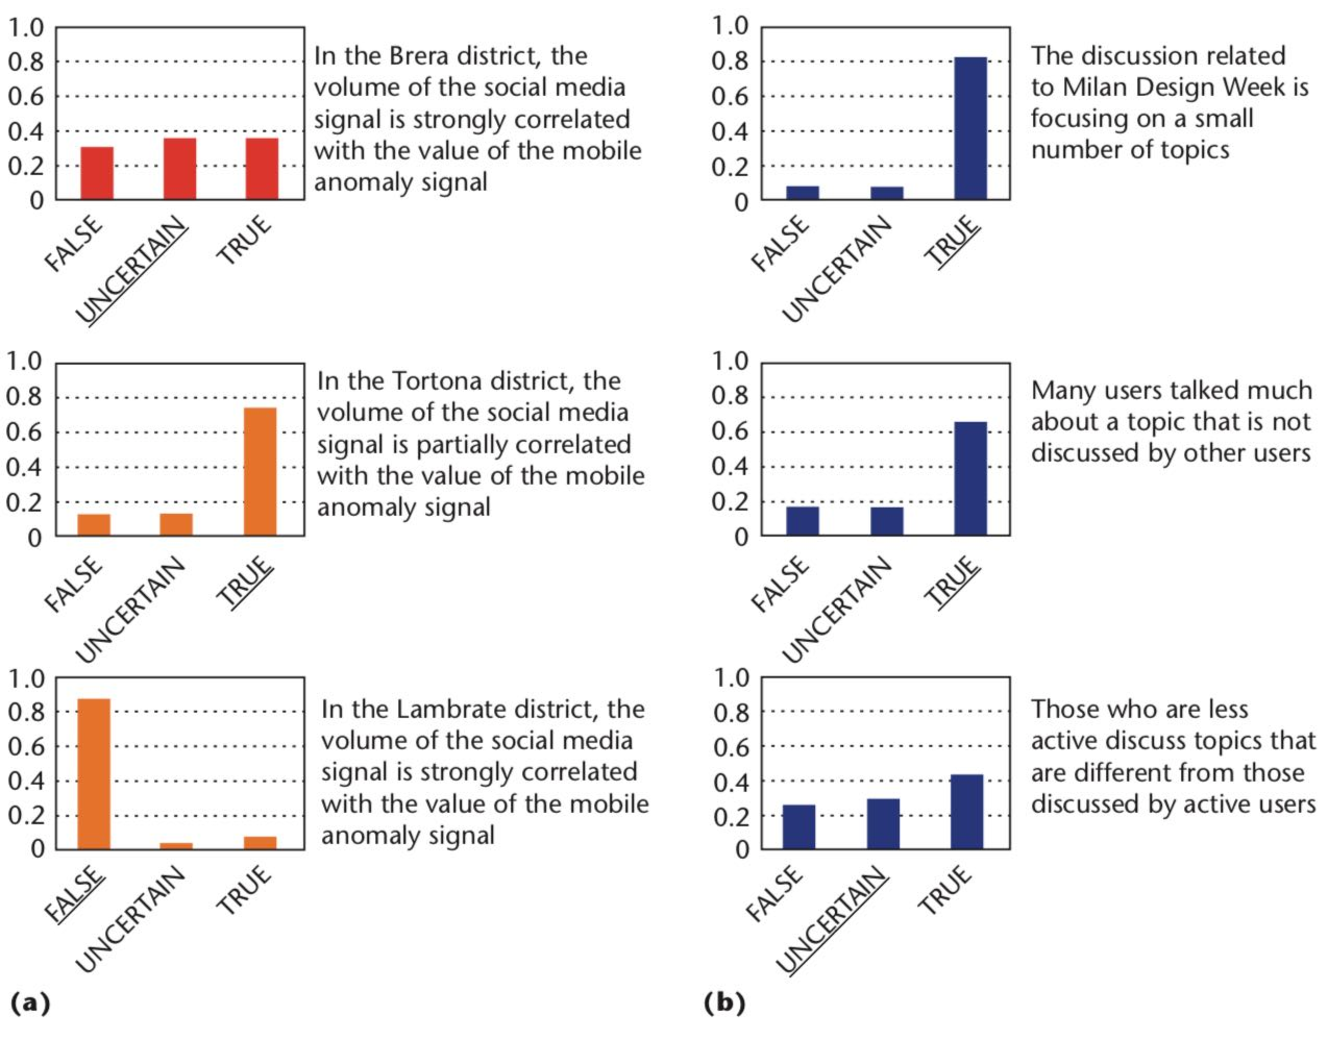
\includegraphics[width=.9\linewidth]{img/mdw-vis-7}
\caption{The results of the questionnaire about the visualizations presented in (a) Figure 5 and (b) Figure 7. As we can see from the distribution of the answers of the 23 responders, the messages we intended to transmit (underlined) were correctly guessed. (source~\cite{DBLP:journals/ieeemm/BalduiniVALAC15}).}
\label{fig:eval-empirical-quest}
\end{figure}

\subsection{MDW2016 - Advanced Visualizations} \label{sec:cs-mdw-2016}
Comforted by the guessability level of the CitySensing visualization, we try to reach an higher level of complexity in the data presentation.
During the 2016 edition of the event we had the opportunity to collect data coming from an additional relevant source: the official mobile application of Fuorisalone. In particular, we had access to the GPS positions of \textsf{place}s where the users open the App and the \textsf{event}s inserted in the agenda on the App. Also, in this context, we apply the method of squared \textsf{grid} tessellation of the city, in order to analyze the correlation between pairs of different signals.

The Figures~\ref{fig:gps_geo_1} and Figures~\ref{fig:gps_geo_2} depicts the results, obtained exploiting \frappe{}, \sti{} and \sparkdi{}, of different use cases that involves data from heterogeneous sources (i.e., GPS record of the usage of the official Fuorisalone App, public social network, official schedule of Fuorisalone events).

\begin{figure}[p]
\centering
\subfloat[]{
	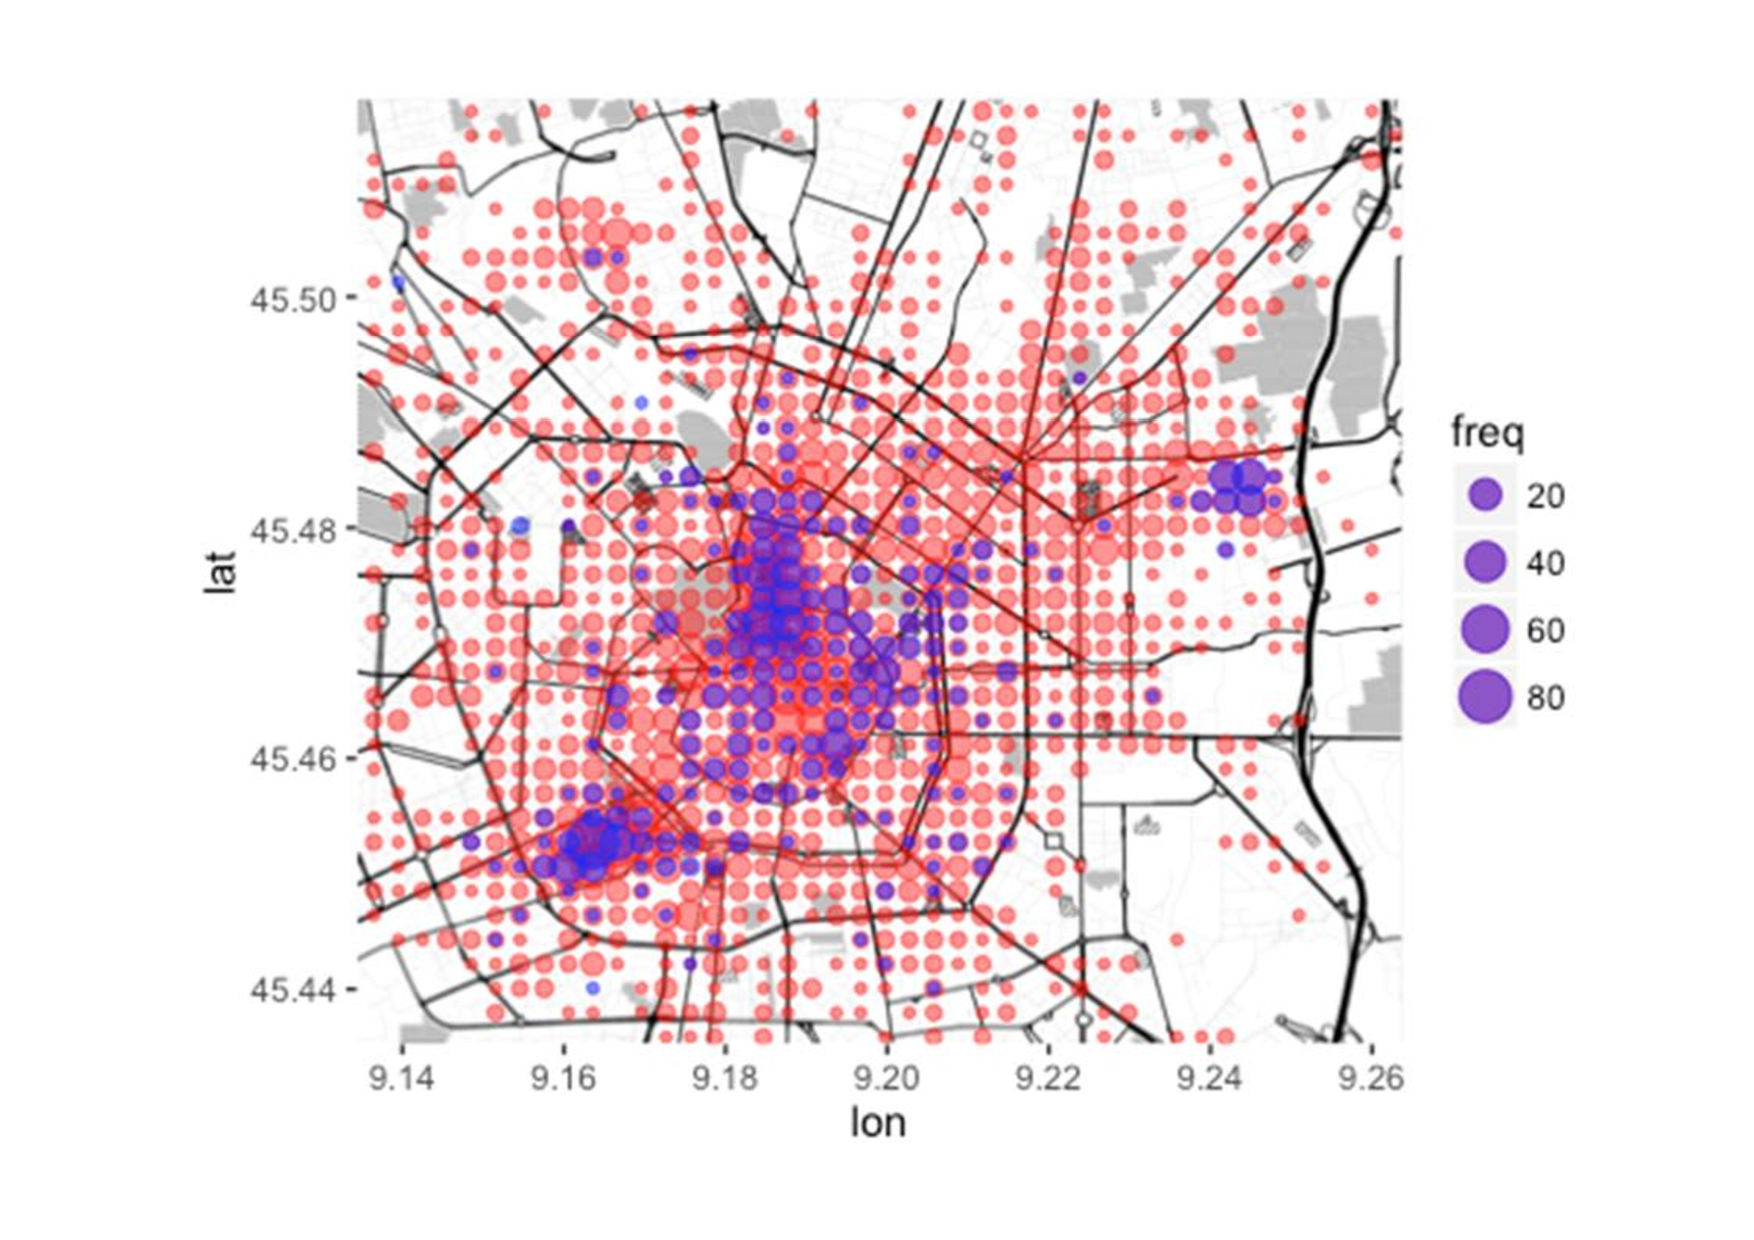
\includegraphics[width=0.75\textwidth]{img/mdw-gps-events} 
} \\
\subfloat[]{
	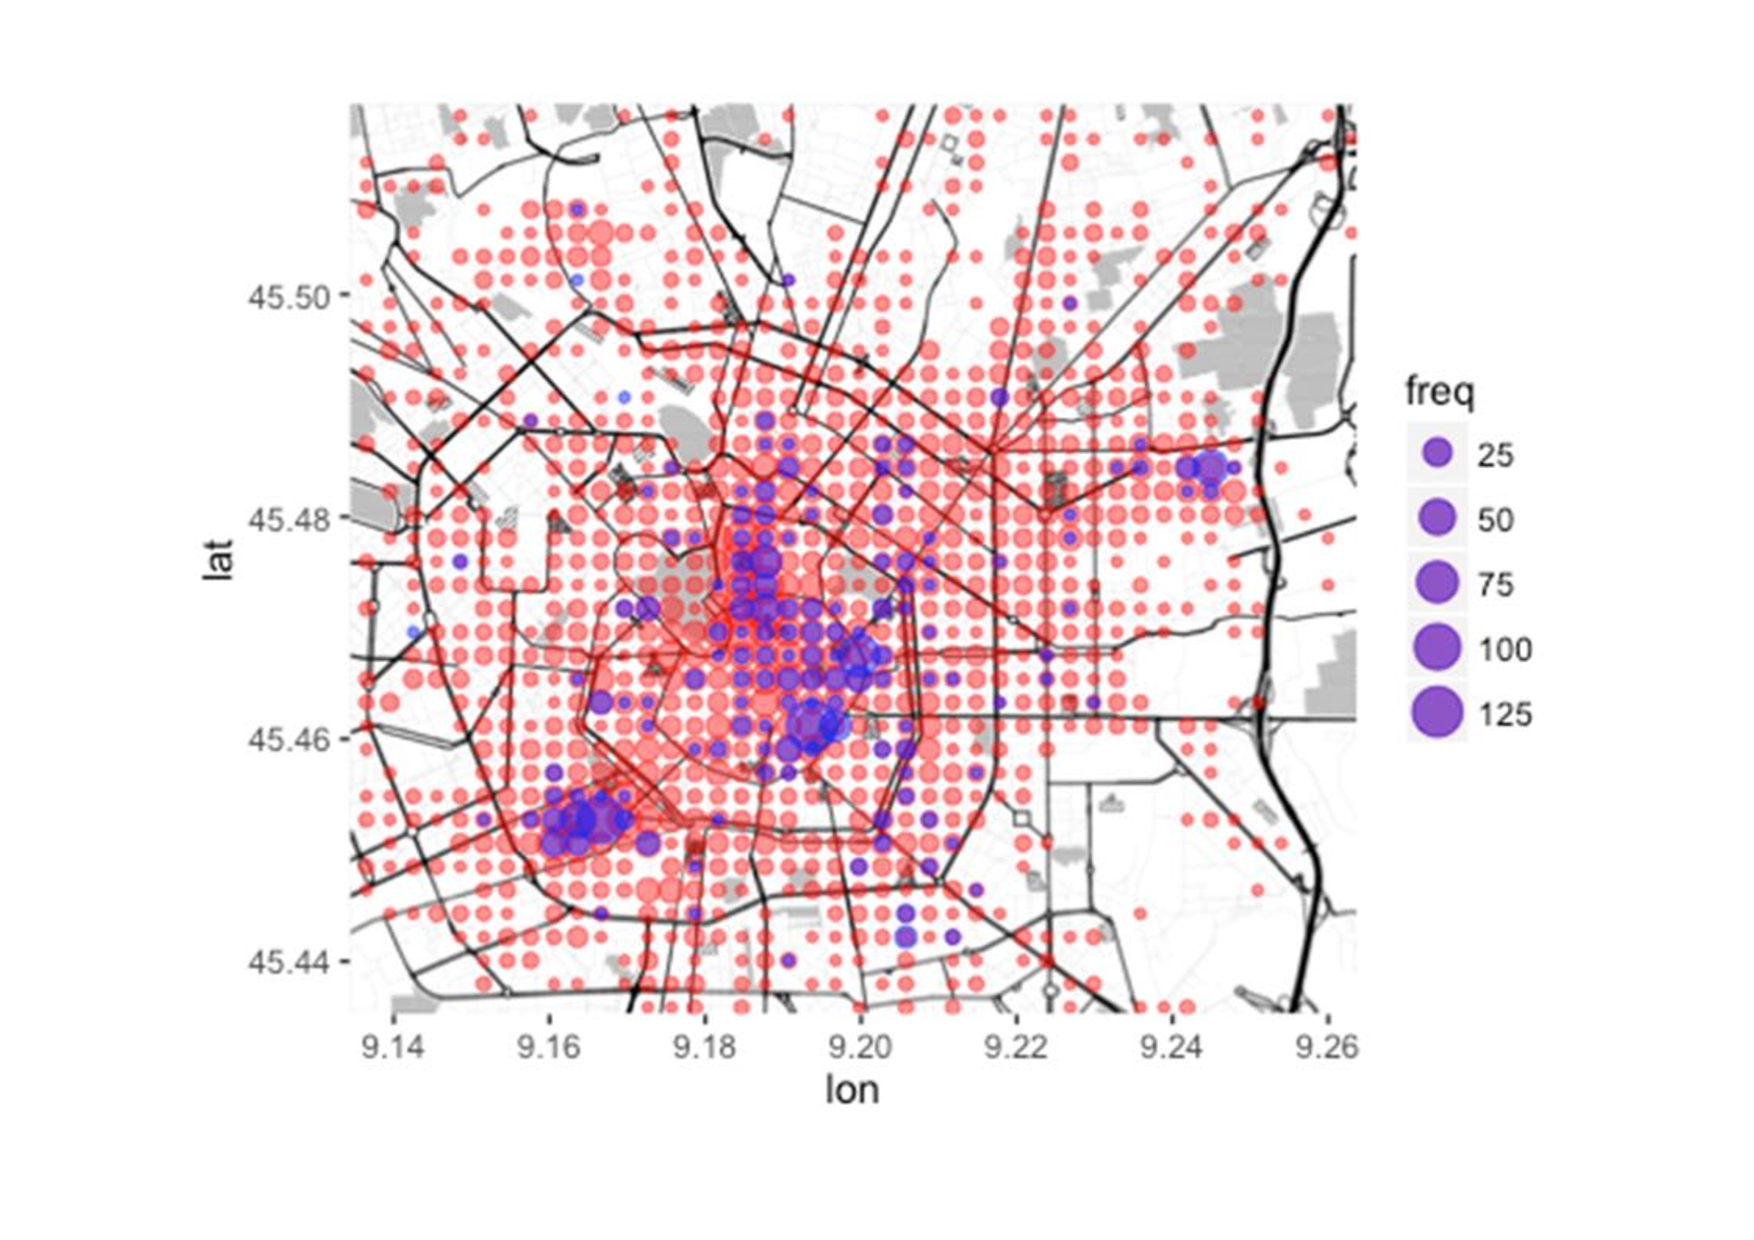
\includegraphics[width=0.75\textwidth]{img/mdw-gps-geo} 
}
\caption{The Figure (a) shows the number of Mobile App GPS observations collected in one day inside each square
of the grid (red dots) correlated with the number of events of Milano Design
Week scheduled for the same day in the same square. The Figure (b shows the correlation between GPS observations (red dots) and geo-located posts on social networks (blue dots) inside each square.}
\label{fig:gps_geo_1}
\end{figure}

Figure~\ref{fig:gps_geo_1}(a) shows the correlation between the use of the App and the number of Fuorisalone events. To visualize such a phenomenon, we consider as \textsf{event}s the use of the App in a \textsf{place}, that generates a GPS record, and the scheduled \textsf{event} of MDW with their \textsf{place} that users put in their agenda. Data is aggregated grouping by \textsf{Pixel}s and capturing daily \textsf{Frame}s.

Another available source of \textsf{Event}s is the geo-located activity on the public social networks: we collect the Twitter and Instagram posts geo-located in the \textsf{Place}s contained in each \textsf{Cell} and we aggregate them gropuping by \textsf{Pixel}s containing the GPS observations, as shown in Figure~\ref{fig:gps_geo_1}(b).
Both \textsf{Frame}s show the increasing of the \textsf{Event}s in the areas of the Fuorisalone.

\begin{figure}[p]
\centering
\subfloat[]{
    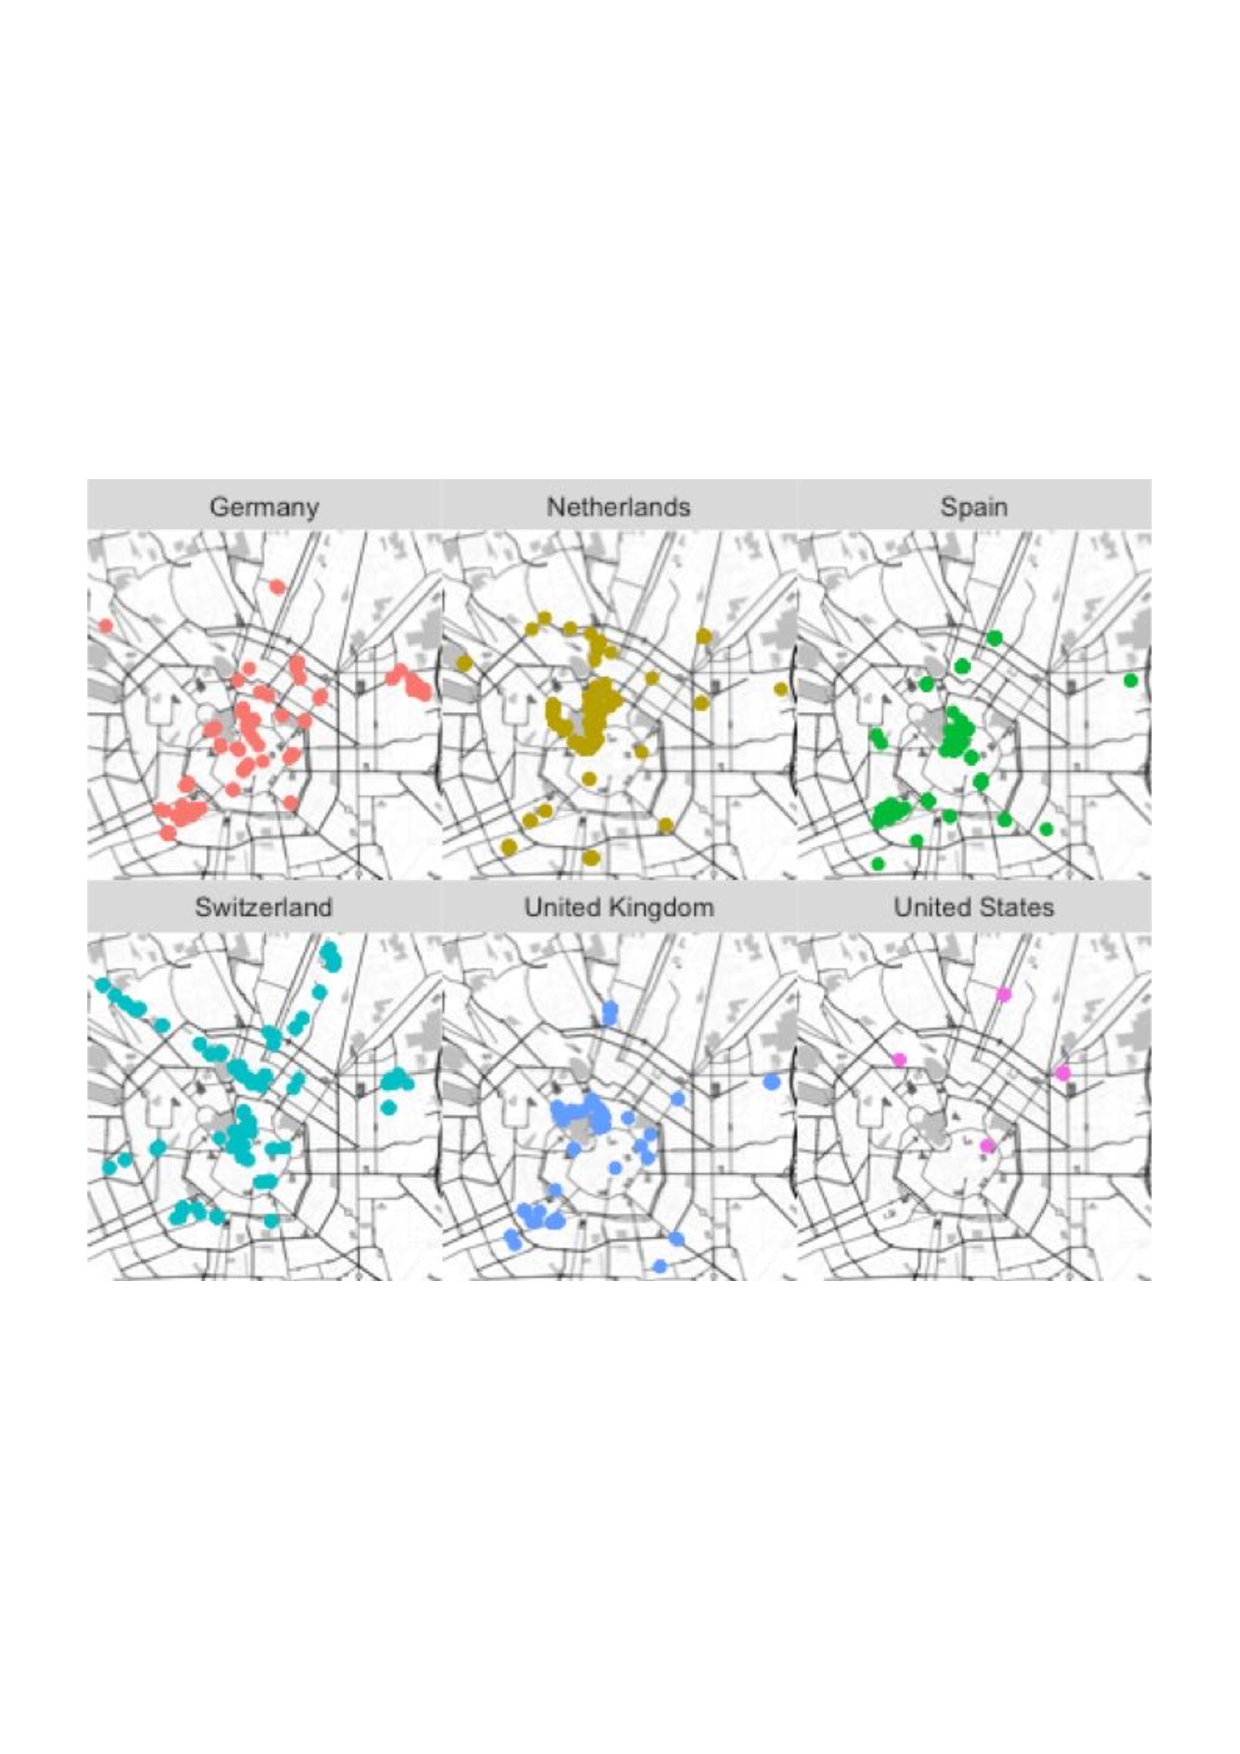
\includegraphics[width=0.75\textwidth]{img/mdw-euro-us-visitors} 
}\\
\subfloat[]{
    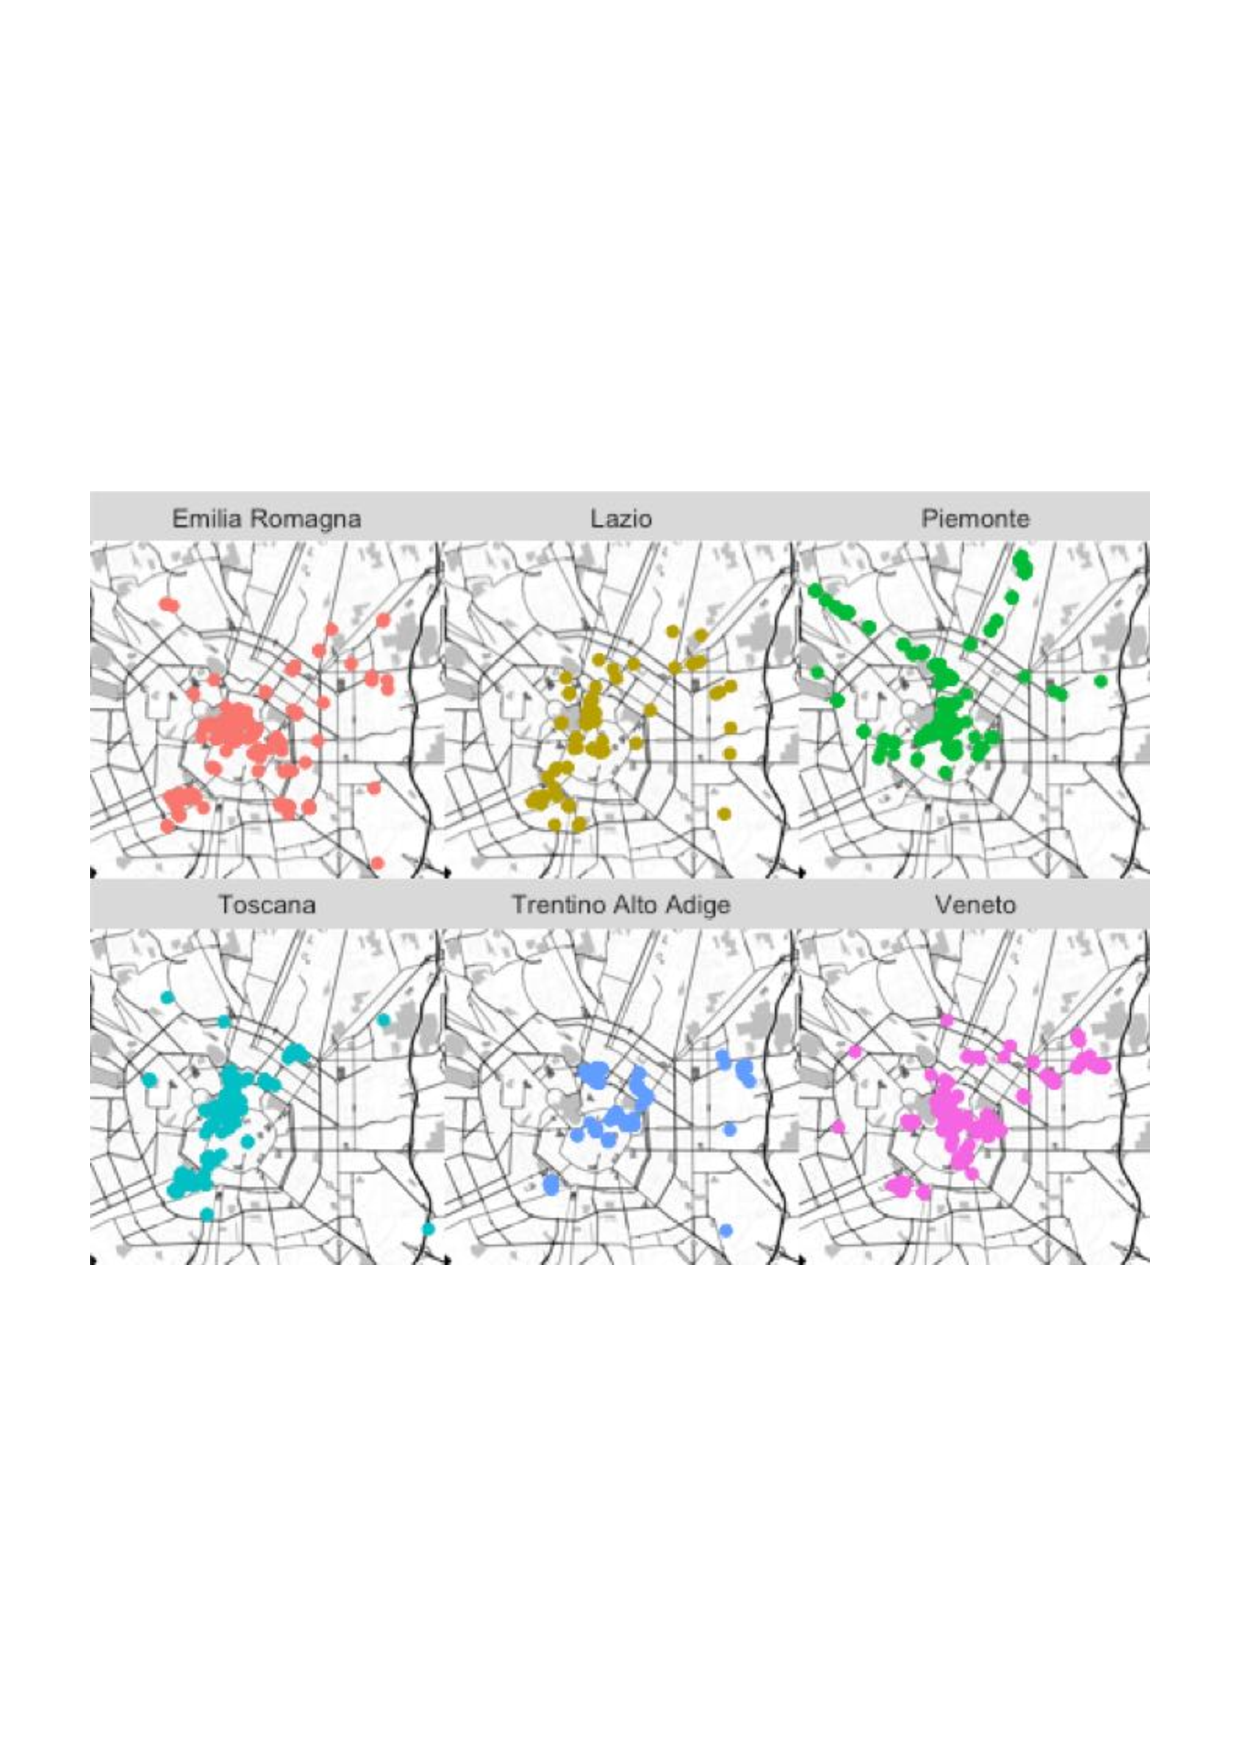
\includegraphics[width=0.75\textwidth]{img/mdw-italian-visitors}
}
\caption{ The Figure presents (a) the localization of the five largest groups of European and US visitors and (b) Italian visitors.}
\label{fig:gps_geo_2}
\end{figure}

Another interesting use case is represented by the analysis of the provenance of the visitors during the Milano Design Week.
In order to estimate the provenance of the visitors we use the GPS information collected by the App, extracting the GPS position of the first observation logged for each user before the days of the MDW (assuming that the users download the App at home). Using appropriate shape files we map each GPS location to a Country in the world, obtaining the provenance of the user.

Mapping the GPS observation \textsf{event}s in the \textsf{grid} of \textsf{pixel}s, it is possible to visualize, for each daily \textsf{frame} and for each people group, which are the most popular areas of the city. Figure~\ref{fig:gps_geo_2}(a) shows the localization of the five largest groups of European foreign visitors and United States visitors. Figure~\ref{fig:gps_geo_2}(b) shows the region of provenance of Italian visitors and their distribution in the events.

As for the public installation during MDW2014, we test the guessability of the advanced visualizations.
The new advanced visualizations are created for a more professional audience (i.e. Studiolabo\footnote{http://studiolabo.it/}, the main organizer and stakeholder of Fuorisalone).
A user-centric study we conducted observing how Studiolabo used the visualizations during a workshop, allowing us to affirm that our stakeholder was able to understand the visualizations and exploit the analysis results.
Therefore, these empirical evaluation of the MDW2016 visualizations enforces the validity of Hypotheses \textsf{Hp.3}.

\section{Milano Fashion Week} \label{sec:cs-mfw}
The Milano Fashion Week (MFW) represents another example of CSE in Milan. This experience deals with the problem of understanding the social media response of the MFW  occurred from the 24$^{th}$ to the 29$^{th}$ February of 2016.
We use \sti{} to analyze the behavior of users who re-acted (or pro-acted) in relationship with each specific fashion show during the week. MFW represents the most important meeting between market operators in the Italian fashion industry. Out of the 170 shows, we are interested only in the catwalk shows, which are the core of the fashion week. The whole set of catwalks includes a total of 73 brands; among them, 68 brands organize one single event, 4 brands organize 2 events, and 1 brand organizes 3 events. 

\begin{figure}[p]
\centering
\subfloat[Granger Causality tests result]{
	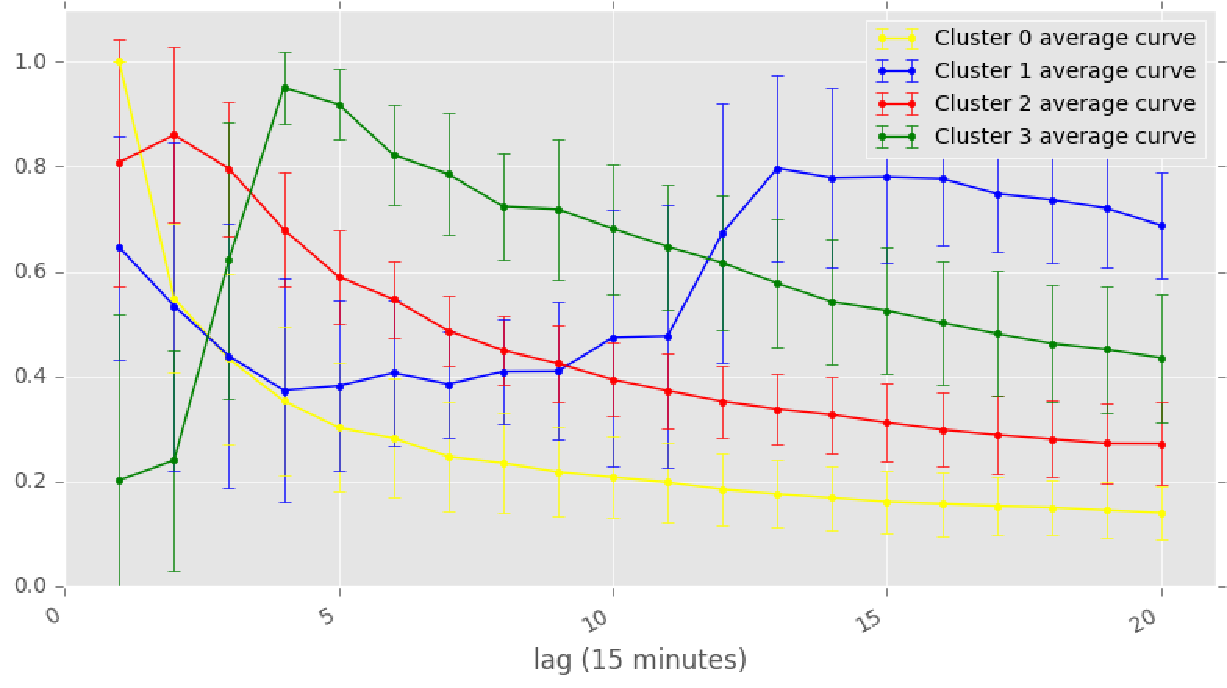
\includegraphics[width=.85\linewidth]{img/mfw-trend}
}\\
\hspace{5pt} 
\subfloat[Density of posts]{
	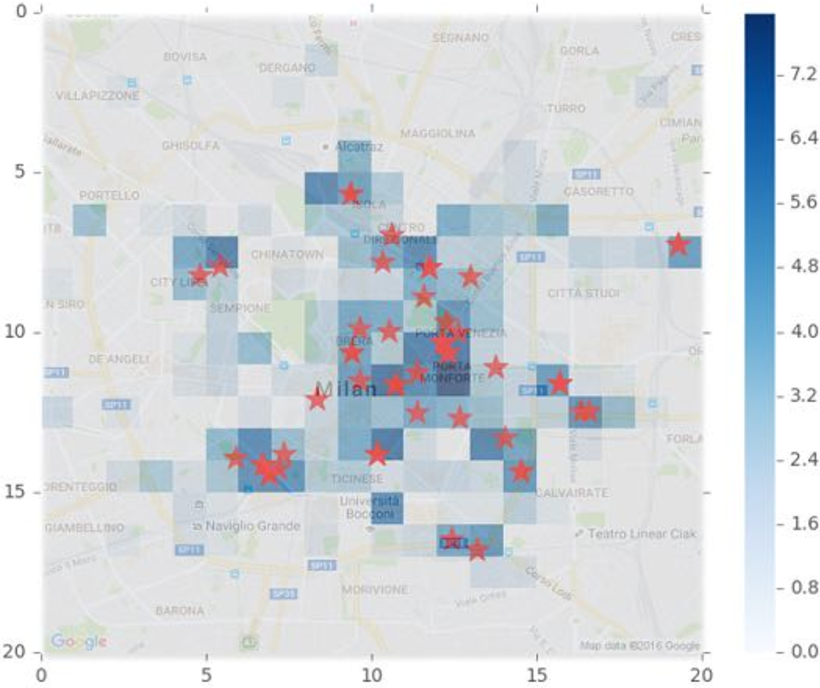
\includegraphics[width=.65\linewidth]{img/mfw-map}
} 
\caption{(a) Granger causality test curves between physical events and social media response of each brand during the MFW, clustered by similarity of behavior; (b) Geographical dispersion over the cells of physical events (red stars)
and density of social media activity (blue).}
\label{fig:fashion_fig}
\end{figure}

We initially extract posts by invoking the social network APIs of Twitter and Instagram; for identifying the social reactions to MFW, we use a set of 21 hashtags and keywords provided by domain experts in the fashion sector, i.e., researchers of the \textit{Fashion in Process} group (FIP) of Politecnico di Milano\footnote{\url{http://www.fashioninprocess.com/}}.
We focused on 3 weeks: the one before, the one after and the one of the event. In this way, \sti{} and \hivedi{} collected 106K tweets (out of which only 6.5\% geo-located) and 556K Instagram posts (out of which 28\% geolocated).
Eventually, we opt for considering only Instagram posts, as they represent a much richer source for the particular domain of Fashion with respect to Twitter~\cite{Brambilla2017, BrambillaSpatial2017}.

We model the data using \frappe{} and exploit \sti{} and \hivedi{} to enable temporal, spatial and content analyses on the modeled information.
Following the \frappe{} approach, we build a regular \textsf{Grid} of \textsf{cell}s above the area of Milan, and assigned each post to the appropriate \textsf{Cell}. The \textsf{Grid} has a square shape, with sides of $10km$, divided into 20 rows and 20 columns, for a total of 400 \textsf{Cell}s of $500m \times 500m$. 

According to the \frappe{} model, an \textsf{Event} is organized by a brand at time $\tau_{n}$, hosted in the \textsf{Place}, located the \textsf{Cell} of a \textsf{Grid}. Each \textsf{Cell} is related to a \textsf{Pixel} and the \textsf{Grid} is captured by a \textsf{CapturedFrame}. An \textsf{Agent} (a user) may contribute with some \textsf{OriginalContent} (e.g., Instagram post), related to an \textsf{Event}, which in turn is going to be augmented by an automated enriching and analysis process that may add entities, as well as extract visual properties (color, pattern, ...) and concepts (objects, people, ...) from posted images.

We extend \frappe{} with \textsf{FrameLevelSynthesis} and \textsf{PixelLevelSynthesis} activities in order to represent the augmentation activities on the \textsf{OriginalContent}. We also add further concepts to \frappe{}.
We name \emph{Alive pixels} those where the percentage of posts shared in the considered pixel is more than $1\%$ of the total number of posts in the frame. We name \emph{Active pixels} those where the percentage of posts shared in the considered pixel is more than $10\%$ of the total number of posts in the frame. We name \emph{Strongly Active pixels} those where the percentage of posts shared in the considered pixel more than $20\%$ of the total number of posts in the frame.
We compute the number of alive, active and strongly active cells for all brands; we also compute the differences between subsequent durations (e.g. 3h - 6h) by counting how many cells changed their state.

Our first goal is to perform a \textbf{temporal analysis} aiming at characterizing the time at which social media respond to the events which appear in the official calendar and are linked to specific brands. 
Exploiting frame level synthesis we observe either peaks of reactions which then quickly disappear, or instead slower reactions that tend to remain observable for a longer time. Estimating the time latency of social responses to events is important for the brands, which could reactively plan more accurate reinforcement actions, essentially by adding well-planned social actions so as to sustain their social presence over time. We run Granger causality for each brand to compare the physical events and the social media reaction, and then we exploite k-means algorithm to cluster the brand by similarity of the Granger curves.
Figure \ref{fig:fashion_fig}(a) shows the clusters of Granger causality curves of the brands.

Our second goal is to \textbf{analyze the geographical dispersion} of social media response. We have two different spatial signals: (i) the calendar events; and (ii) the volume of social media posts on the Web with geographical information attached, i.e., latitude and longitude. Given these two signals, several features can be computed in order to describe the spatial dispersion of posts following an event. 
We compute different measures that reflect the dispersion of the social media signal over time, using: \emph{Gini coefficient}, \emph{Average distance} of the social media signals from the event location, and the number of \emph{alive}, \emph{active} and \emph{strongly active} cells.
Figure~\ref{fig:fashion_fig} (b) shows the  map representing the geographical distribution of events (represented by red stars) and post density using a synthetic frame where the pixel are darker where the density is higher.

The final result of the analysis is a set of advanced visual interfaces to be exploited by professional users.
The stakeholder (FIP), exploiting those visual interfaces, was able to observe that: (i) as the duration of the frame increases, the number of \emph{alive pixels} also increases. Moreover, the number of \emph{active} and \emph{strongly active pixels} is floating in the range from 1 to 3, with very few brands reaching 4 \emph{active pixels}. (ii) At the start of the event, posts are shared near the event location, but, as looking at the bigger picture, including 24 hours or even the entire period of 24 days, the \emph{average distance} is increasing, showing the growing dispersion of the social signal. (iii) The \emph{Gini coefficient} proves how the concentration of the social signal remains always high, due also to the fact that the low percentage of users that allows Instagram to geo-tag their own photo is reducing the number of authors implied in this study, and so the few authors with high volumes of posts generated are biasing the results. However, looking at the \emph{Gini alive coefficient}, which refers to the Gini coefficient computed only over the pixels that result alive for at least one brand in the specific frame, they can see a weak smoothing of the concentration strength with the increasing of the time-scope.

This proposed visual interfaces, based on \frappe{} concept (in particular, Frame and Pixel), result guessable and enable visual correlation of the presence of an event (stars) to the density of the social activity (darker pixels) over time.
The guessability of this visualizations validates, once more, Hypothesis \textsf{Hp.3}.

\section{Como Smart City for Smart Citizens} \label{sec:cs-como}
Como Smart City for Smart Citizens (ComoSC\textsuperscript{2}) is a big-data integration project started in 2016 where we involve the Municipality of Como and TIM-Telecom Italia. The purpose of the project is to create a system for the integration, analysis and interpretation of the large amount and heterogeneous data coming from different sources, in order to understand Como's urban dynamics and support  the decision making process of Como's local government.

\begin{figure}[t]
  \centering
  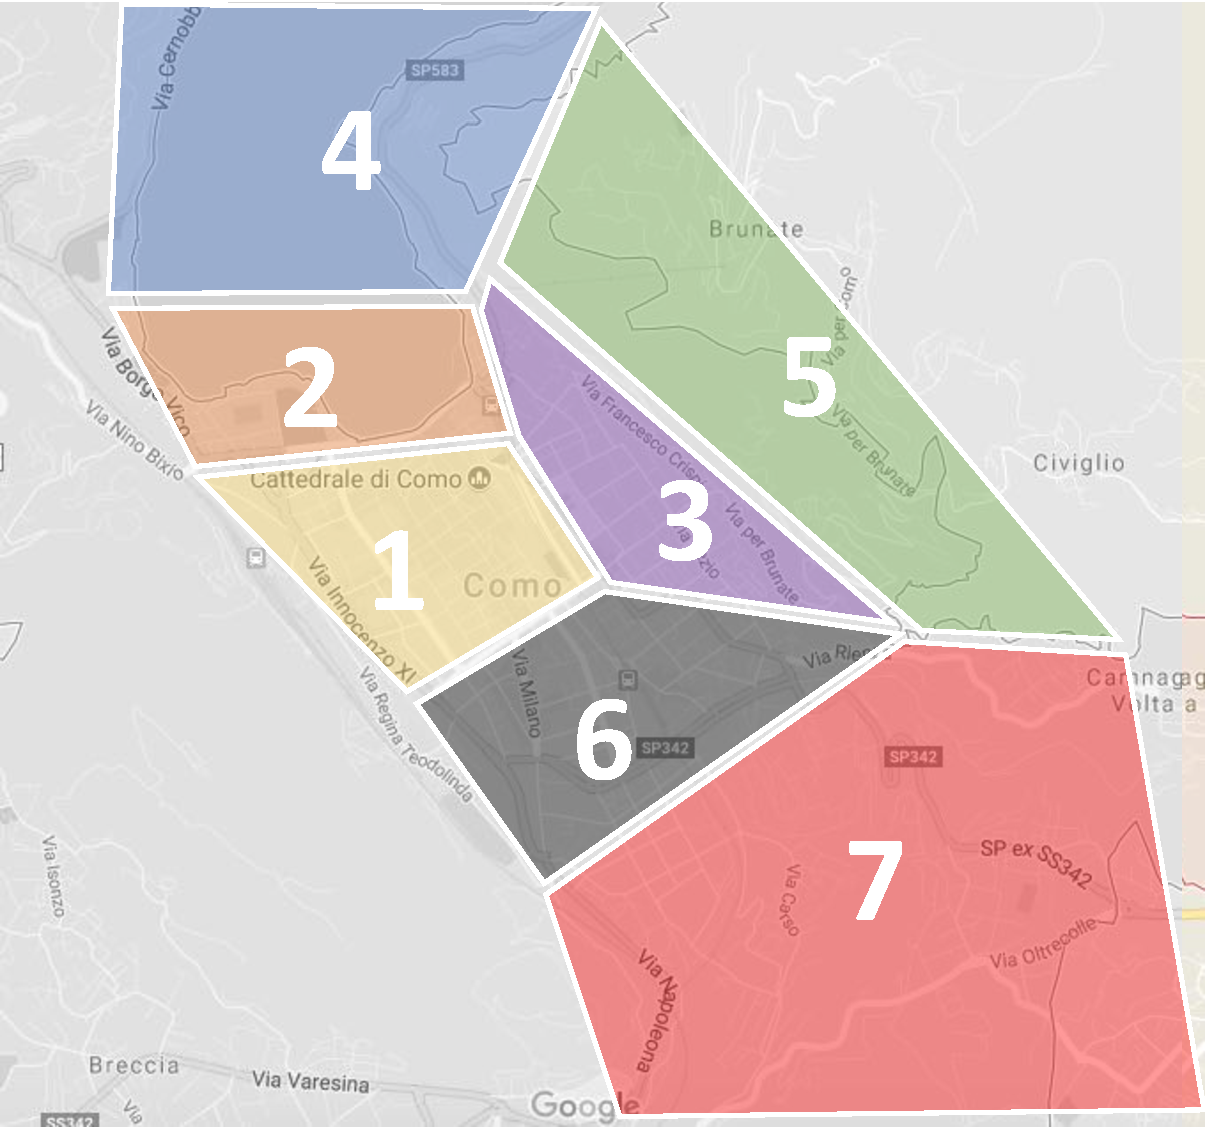
\includegraphics[width=.6\linewidth]{img/como-district}
  \caption{The seven irregular data-driven cells based on mobile phone data that cover the Como territory.}
  \label{fig:map1}
\end{figure}

As in MDW, we analyze the dynamics of \textbf{mobile phone traffic} (preventively anonymized and aggregated, according to privacy-preserving policies) in different areas of the city. 
Differently from the experiences in Section~\ref{sec:cs-mdw}~and~\ref{sec:cs-mfw}, in ComoSC\textsuperscript{2} we use \frappe{} with and irregular \textsf{Grid} composed by seven data-driven \textsf{cell}s built according to the distribution of the phone antennas and the characteristics of the area. 
We name those cells: historical city  center, lakeside promenade, touristic areas outside from the historical center, lake area, mountain area around the city, business and universities area, industrial outskirts.
The map in Figure~\ref{fig:map1} represents the distribution of the seven cells.

% One example is the comparison between the number of visitors from neighboring countries of Italy. 
% As depicted in Figure~\ref{fig:como_country_day}, Swiss people usually comes to Como for shopping on Saturdays in July while this trend dramatically decreases in September. 

\begin{figure}[p]
\centering
\subfloat[]{
        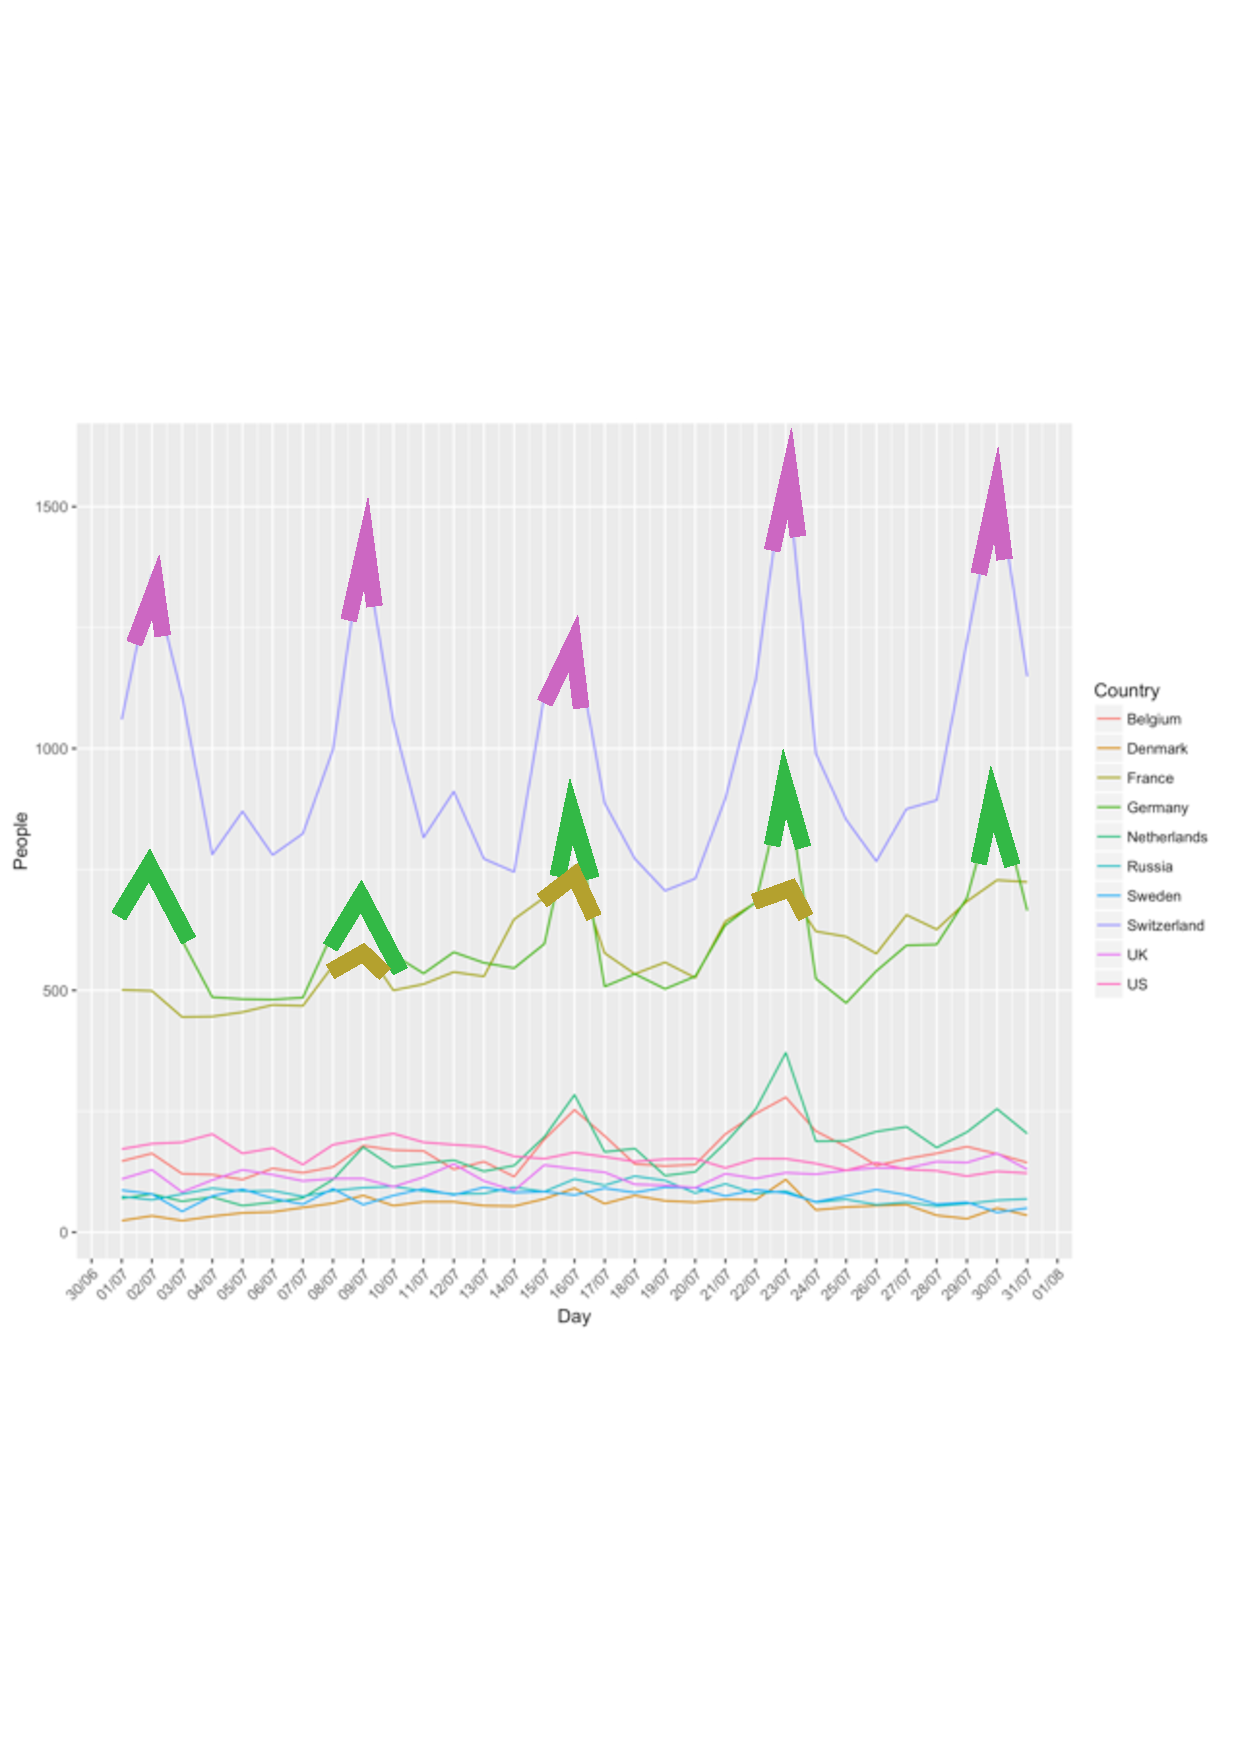
\includegraphics[width=.75\linewidth]{img/como-visit-july}
}\\
\subfloat[]{
        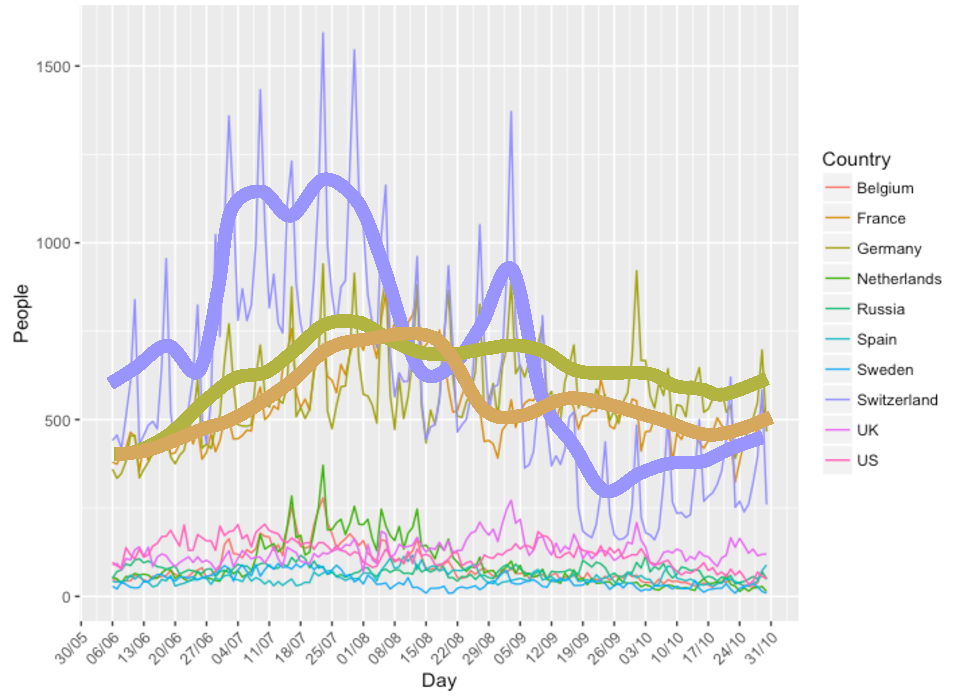
\includegraphics[width=.75\linewidth]{img/como-visit-summer}
}
\caption{(a)Number of foreign visitors per country per day in July in Como: Swiss, German, and French are the most present in the weekends. (b) Number of foreign visitors per country per day in Como from June to October. One can notice that Swiss visitors decrease sensibly in September.}
        \label{fig:como_country_day}
\end{figure}

We collect the mobile phone traffic data during several months, in particular we focuse on the summer period (from May to October 2016). Inside each \textsf{cell}, exploiting \sparkdi{}, we analyze the trend of mobile phone traffic capturing \textsf{frame}s with different duration (one hour, one day) and different coverage (the complete grid or a group of cells). 
Anonymized mobile phone data contains also information about the SIM (like international dial-code) and demographics information about the owner of the SIM (like gender or age-range).
As a result, we can perform analysis not only about the \textsf{event}s of people presence but also about the characteristics of people (\textsf{event content}) and to produce visualizations to ease the understanding of complex data.
For instance, Figure~\ref{fig:como_country_day} shows the comparison between the number of visitors from neighboring countries of Italy.
In particular Figure~\ref{fig:como_country_day}(a) shows the amount of visitors during the summer, while Figure~\ref{fig:como_country_day}(b) refers to July.

\begin{figure} [t]
        \centering
        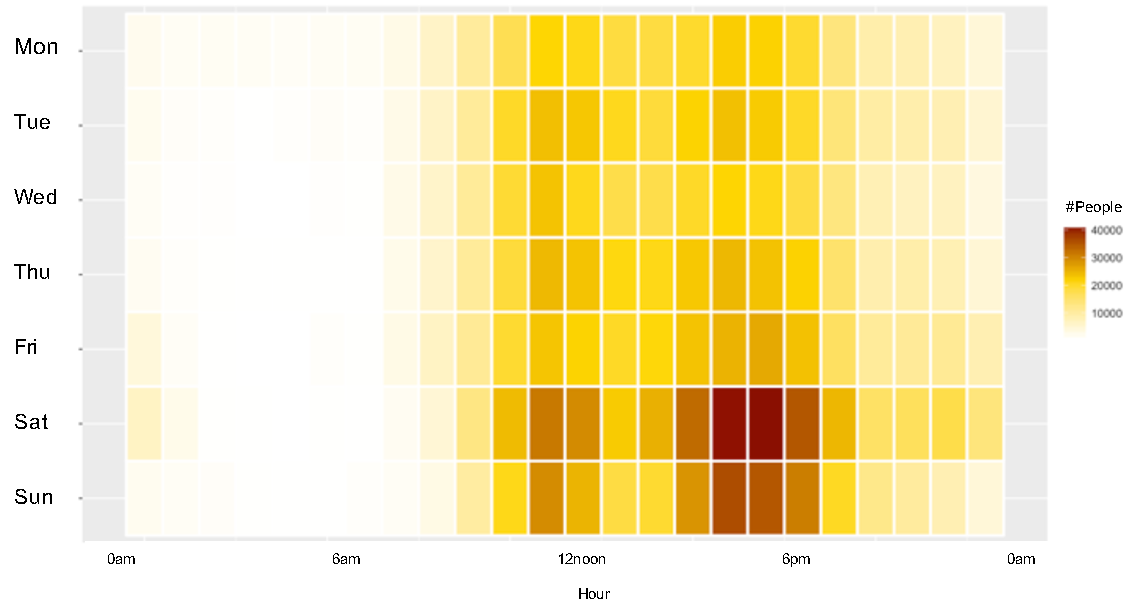
\includegraphics[width=.8\linewidth]{img/como-hourly-distribution}
        \caption{Patterns of people presence in Duomo Square on working days and weekends: Tuesday, Thursday and Saturday are more crowded due to open market in the streets; Week ends are extremely crowded (including Saturday night).}
        \label{fig:duomo}
\end{figure}

Besides mobile phone data analysis, we instrumented the Cathedral Square of Como (\textit{Piazza Duomo}) with a set of \textbf{IoT (Internet of Things) sensors for counting people} passing in the square. The installation of the IoT sensors covers all the access to the square, and each sensor count how many people pass from the access every minute and push the results in real-time to \sparkdi{}.
We collect the data from IoT sensors and model it with \frappe{}.
Exploiting \textsf{CapturedFrames} with different time duration (hour, day and week), we construct the trend of passages \emph{from} and \emph{to} the Duomo Square according to the day of the week and the hour of the day (see Figure~\ref{fig:duomo}). 
This trend represents the starting point to analyze trending pattern and anomalies. 

The result of the analysis is a report containing an overview of the crowd movement around the city.
In order to validate Hypothesis \textsf{Hp.3}, we organized a workshop for the data analysis team of the Municipality of Como.
Exploiting the report on the analysis of mobile traffic data, the analysts were able to identify particular trends. For instance, the analysis of Figure~\ref{fig:como_country_day} shows that Swiss people usually comes to Como for shopping on Saturdays in July, but this trend dramatically decreases in September.
Moreover, exploiting the passage trend analysis, the team, identifies two different patterns of people presence in Duomo Square: one for working days and one for weekends, with a significant increase of people during Saturdays and Sundays, with respect to working days.
More in details, they found some differences inside the two patterns. For example in week-ends clearly emerge a difference during the evenings: Saturday evening shows a sort of persistence of people presence, while Sunday evenings appear more similar to working-day evenings. Another significant difference is the increase of people presence on Tuesday and Thursday mornings, with respect to the other working days. They are significant because the local market activities in the square during such mornings induces higher flows than usual.

The report eases the access to the results and is exploited by the Municipality of Como to enable decision making process to change the urban aspect of the city center (i.e,  the creation of a new pedestrian zone).
Once again, we collected experimental evidence that the \frappe{} approach, together with the \sparkdi{} implementation of \river{}, enables a series of different analytics on data streams characterized by high variety.
The understandability of complex data and the enabled decision making process validate Hypothesis \textsf{Hp.3}.

\section{Conclusion} \label{sec:cs-conclusion}
In this section, we conclude the chapter by showing the correlation of the case studies with: (i) the adoption and the evolution of the \frappe{} concepts, and (ii) the implementation of \river{} that better fits the analytics needs.
Table~\ref{tab:frappeAnalysis} proposes an analysis of how important each of the \frappe{} concept is in the various experiments and shows the extendibility of \frappe{}, while Table~\ref{tab:techAnalysis} shows which implementation of \river{} is used in the various use case. 

\begin{table}[t]
\centering
\small
\caption{A comparison of how the \frappe{} concepts are used in the two large-scale events of Milan Design Week (MDW) and Milan Fashion Week (MFW) as well as in a longitudinal analysis we performed Como. The `x' symbols have the following meaning: xxx -- key concept; xx -- important concept; and x -- useful concept. The lack of stars means that the concept was not used.}
\label{tab:frappeAnalysis}
\begin{tabular}{@{}llccccccccclcl@{}}

\toprule
                          &                       & MDW                                      & MFW                 & Como \\ \midrule
\parbox[t]{1mm}{\multirow{3}{*}{\rotatebox[origin=c]{90}{Spatial}}}  & Place                 & \cellcolor[red]{.5}xxx               & xxx                &      x              \\
                          & Cell                  & \cellcolor[HTML]{EFEFEF}xx                & x                  & xx   \\
                          & Grid                  & \cellcolor[HTML]{EFEFEF}x                 & x                  & xx   \\ \midrule
\parbox[t]{1mm}{\multirow{5}{*}{\rotatebox[origin=c]{90}{Temporal}}}  & Event                 & \cellcolor[HTML]{EFEFEF}xxx               & xxx                &  x   \\
                          & Pixel                 & \cellcolor[HTML]{EFEFEF}xx                & x                  & xx  \\
                          & Frame                 & \cellcolor[HTML]{EFEFEF}x                 & x                  & xx  \\
                          & - CapturedFrame       & \cellcolor[HTML]{EFEFEF}xx                &                    & xxx \\
                          & - SyntheticFrame    &\cellcolor[HTML]{EFEFEF}xx                &                    & xxx  \\ \midrule
\parbox[t]{1mm}{\multirow{5}{*}{\rotatebox[origin=c]{90}{Content}}}  & Content   & \cellcolor[HTML]{EFEFEF}xxx                 & x                &    \\
                          & - Event-level content   &                  & \cellcolor[HTML]{EFEFEF}xxx                &   x   \\
                          & ~~~- Original content    &                  & \cellcolor[HTML]{EFEFEF}xxx               &  x    \\
                          & ~~~- Augmented content   &                & \cellcolor[HTML]{EFEFEF}xx                  &  x    \\
                          & - Pixel-level synthesis &                & \cellcolor[HTML]{EFEFEF}xxx                & xxx     \\
                          & - Frame-level synthesis &                   & xx                    & \cellcolor[HTML]{EFEFEF}xxx   \\ \midrule
\parbox[t]{1mm}{\multirow{4}{*}{\rotatebox[origin=c]{90}{Provenance}}}                & Action                &   \cellcolor[HTML]{EFEFEF}x                &                    &       &   \\
                          & - Capture             &                  & \cellcolor[HTML]{EFEFEF}x                          & xx   \\
                          & - Synthesize          &                 & \cellcolor[HTML]{EFEFEF}xx                         & xx    \\
                          & - Augment             &                 &  \cellcolor[HTML]{EFEFEF}xx                        & xx     \\ \bottomrule
\end{tabular}
\end{table}

\begin{table}
\centering
\caption{An overview of analysis technologies used in the two large-scale events of Milan Design Week (MDW) and Milan Fashion Week (MFW) as well as in a longitudinal analysis we performed Como.}
\label{tab:techAnalysis}
\begin{tabular}{@{}llccccccccclcl@{}}
\toprule
& & MDW2013 & MDW2014 & MDW2016 & MFW & ComoSC\textsuperscript{2} \\ \midrule
\parbox[t]{1mm}{\multirow{4}{*}{\rotatebox[origin=c]{90}{}}} & SLD                     & x & x &   &   &   \\
                          & \sti{}                   &   &   & x & x &   \\
                          & \hivedi{}                &   &   & x & x &   \\
                          & \sparkdi{}               &   &   & x &   & x \\ \midrule
\end{tabular}
\end{table}

The basic \frappe{} concepts were introduced during the Milan Design Week experiences. The accent is on \emph{Place} and \emph{Event}. Also the \emph{Cell} and the  \emph{Pixel} -- its time-variant counterpart -- are important to bridge the gap between the analyzed data and the visual analytics we intend to enable~\cite{DBLP:journals/ieeemm/BalduiniVALAC15}. The \emph{Grid} and  \emph{Pixel} -- its time-variant counterpart -- were useful as abstractions, but they did not play a key role. The provenance of all steps of the analysis were documented using the generic \emph{Action} concept; captured and synthesized were only possible value of an attribute of the action. 
The data of the MDW2013 and MDW2014 experiences, is analyzed using SLD (see Section~\ref{sec:sld}), while the MDW2016 is the first real world validation for the \textit{lazy transformation} approach implemented in \sti{}, and for the distributed implementations of \river{} in Spark and HIVE. 
Indeed, during the 2016 edition, the data from telco network (CDR) is characterized by an high volume, so we first aggregate it using \sparkdi{} and \hivedi{} implementations of \river{}. \sti, instead, is used to analyze social network data, enrich it and merge the different data aggregations.

The Milano Fashion Week experience is key to extend the original \frappe{} with the concepts that allow describing the content as well as to extend \frappe{} with some provenance concepts. Specifically for this experience, in \frappe{} 2.0.we introduce the distinction between \emph{original} and \emph{augmented} content at \emph{event-level}. We also perceive the need to model the content that we connected to each pixels, namely the \emph{pixel-level synthesis}. We reflecte this extension also in the provenance part of \frappe{} introducing the \emph{capture}, the \emph{augment} and the \emph{synthesize} actions. The data of the MFW was analyzed exploiting \sti{} and \hivedi{}.

The longitudinal analysis, which we performed on Como in the context of ComoSC\textsuperscript{2}, serve as validation for \frappe{} 2.0. All the concepts are used, although their use and benefit depends on the different types of analysis performed. In particular, more emphasis is posed on the \emph{Grid}, the \emph{Frames} and the \emph{frame-level synthesis}, which is introduced in \frappe{} during this experience. 
The data involved in the Como experience, in particular the demographically enriched CDR, must be pre-aggregated in order to manage its volume. We exploit \sparkdi{} to perform this task and to aggregate the results.

The experiences in Milan (MDW and MFW) and in Como demonstrate the validity of the \frappe{} approach in the data representation, and the robustness of the implementations of \river{}.
The guessability of the data visualizations improved the understanding of the urban environment from different points of view and enabled decision making processes by the stakeholders.
The results of these experiences validate Hypothesis \textsf{Hp.3}.